\documentclass[PhD]{msu-thesis}

% \pdfoutput=1

% \usepackage[utf8]{inputenc} % allow  utf-8 inpute
\usepackage[T1]{fontenc}    % use 8-bit T1 fonts
% \usepackage{lmodern}        % to have \textasciitilde vertically centered
% \usepackage{hyperref}       % hyperlinks
% \usepackage{url}            % simple URL typesetting
% \usepackage{booktabs}       % professional-quality tables
% \usepackage{amsfonts}       % blackboard math symbols
% \usepackage{amssymb}
% \usepackage{amsmath}
% \usepackage{bm}
% \usepackage{units}
% \usepackage{nicefrac}       % compact symbols for 1/2, etc.
% \usepackage{microtype}      % microtypography
% \usepackage{lipsum}
\usepackage{xcolor}
% \usepackage{tabularx,caption,booktabs}
% \usepackage{gensymb}
% \usepackage{mathrsfs}
% \usepackage{mathtools}
% \usepackage{xspace}
% \usepackage{multirow}
% \usepackage{afterpage}
% \usepackage{geometry}
% \usepackage{pdflscape}
% \usepackage{arydshln}
% \usepackage[normalem]{ulem}
% \usepackage{lineno}
% \usepackage{authblk}
\usepackage{newtxtext,newtxmath}
\usepackage[capitalize]{cleveref}
\usepackage{dark_matter}
% \linenumbers



\title{Leveraging Multi-Messenger Astrophysics for Dark Matter Searches}
\author{Daniel Nicholas Salazar-Gallegos}
\dualmajor{Physics}{Computational Mathematics in Science and Engineering}
\date{Today}

\begin{document}
\newcommand{\sv}{\langle \sigma \mathit{v} \rangle}

\frontmatter
\maketitlepage

%%%%%%%%%%%%%%%%%%%%%%%%%%%%%%%%%%%%%%%%%%%%%%%%%%%%%%%%%%%%%%%%%%%%%%%%%%%%%%%%%%%%%
\begin{abstract}
    I did Dark Matter with HAWC and IceCube. I also used Graph Neural Networks
\end{abstract}
%%%%%%%%%%%%%%%%%%%%%%%%%%%%%%%%%%%%%%%%%%%%%%%%%%%%%%%%%%%%%%%%%%%%%%%%%%%%%%%%%%%%%

\clearpage

\makecopyrightpage

\clearpage

%%%%%%%%%%%%%%%%%%%%%%%%%%%%%%%%%%%%%%%%%%%%%%%%%%%%%%%%%%%%%%%%%%%%%%%%%%%%%%%%%%%%%
\chapter*{Acknowledgments}
\DoubleSpacing
I love my friends.
Thanks to everyone that helped me figure this out.
Amazing thanks to the people at LANL who supported me.
Eames, etc
Dinner Parties
Jenny and her child Kaydince
Kirsten, Pat, Andrea
Family.
Roommate
%%%%%%%%%%%%%%%%%%%%%%%%%%%%%%%%%%%%%%%%%%%%%%%%%%%%%%%%%%%%%%%%%%%%%%%%%%%%%%%%%%%%%

\clearpage

\SingleSpacing

\tableofcontents*
\clearpage

\listoftables
Proof I know how to include
\clearpage

\listoffigures
Make the figures document at some point...

% \begin{abbreviations}
    % \abbrev{MSU}{Michigan State University}
    % \abbrev{LANL}{Los Alamos National Laboratory}
% \end{abbreviations}

\mainmatter

%%%%%%%%%%%%%%%%%%%%%%%%%%%%%%%%%%%%%%%%%%%%%%%%%%%%%%%%%%%%%%%%%%%%%%%%%%%%%%%%%%%%%
\chapter{Introduction\label{sec:intro}}
%%%%%%%%%%%%%%%%%%%%%%%%%%%%%%%%%%%%%%%%%%%%%%%%%%%%%%%%%%%%%%%%%%%%%%%%%%%%%%%%%%%%%
Is the text not rendering right? Ah ok it knows im basically drafting the doc still

%%%%%%%%%%%%%%%%%%%%%%%%%%%%%%%%%%%%%%%%%%%%%%%%%%%%%%%%%%%%%%%%%%%%%%%%%%%%%%%%%%%%%
\chapter{Dark Matter in the Cosmos\label{sec:dm_cosmos}}
%%%%%%%%%%%%%%%%%%%%%%%%%%%%%%%%%%%%%%%%%%%%%%%%%%%%%%%%%%%%%%%%%%%%%%%%%%%%%%%%%%%%%
%-----------------------------------------------------------------------------------%
\section{Introduction\label{sec:intro2dm}}
%-----------------------------------------------------------------------------------%

The dark matter problem can be summarized in part by the following thought experiment.

Let us say you are the teacher for an elementary school classroom.
You take them on a field trip to your local science museum and among the exhibits is one for mass and weight.
The exhibit has a gigantic scale, and you come up with a fun problem for your class.

You ask your class, "What is the total weight of the classroom?
Give your best estimation to me in 30 minutes, and then we'll check your guess on the scale.
If your guess is within 10\% of the right answer, we will stop for ice cream on the way back."

The students are ecstatic to hear this, and they get to work.
The solution is some variation of the following strategy.
The students should give each other their weight or best guess if they do not know.
Then, all they need to do is add each student's weight and get a grand total for the class.
The measurement on the giant scale should show the true weight of the class.
When comparing the measured weight to your estimation, multiply the measurement by 1.0 $\pm$~0.1 to get the $\pm$10\% tolerances for your estimation.

Two of your students, Sandra and Mario, return to you with a solution.

They say, "We weren't sure of everyone's weight.
We used 65 lbs for the people we didn't know and added everyone who does know.
There are 30 of us, and we got 2,000 lbs!
That's a ton!"

You estimated 1,900 lbs. assuming the average weight of a student in your class was 60 lbs.
So, you are pleased with Sandra's and Mario's answer.
You instruct your students to all gather on the giant scale and read off the weight together.
To all your surprise, the scale reads \textit{10,000 lbs}!
10,000, in technical terms, is significantly more than a 10\% error from 2,000.
In fact, it is approximately 5 times more massive than either your or your students' estimates.
You think to yourself and conclude there must be something wrong with the scale.
You ask an employee to check the scale and verify it is well calibrated.
They confirm that the scale is in working order.
You weigh a couple of students individually to assess for yourself that the scale is well calibrated.
Sandra weighs 59 lbs, and Mario weighs 62 lbs, typical weights for their age.
You then weigh each student individually and see that their weights individually do not deviate greatly from 60 lbs.
So, where does all the extra weight come from?
This dilemma is what we are faced with when weighing the cosmos.

This thought experiment serves as an analogy to the Dark Matter problem.
The important substitution to make however is to replace the students with stars and the classroom with a galaxy, say the Milky Way.
Individually the mass of stars is well measured and defined with the Sun as our nearest test case.
However, when we set out to measure the mass of a collection of stars as large as galaxies, our well-motivated estimation is wildly incorrect.
There simply is no way to account for this discrepancy except without some unseen, or dark, contribution to mass and matter in galaxies.
I set out in my thesis to narrow the possibilities of what this Dark Matter could be.

%-----------------------------------------------------------------------------------%
\section{Dark Matter Basics\label{sec:basicDM}}
%-----------------------------------------------------------------------------------%

Presently, a more compelling theory of cosmology that includes Dark Matter (DM) in order to explain a variety of observations is $\Lambda$ \textbf{C}old \textbf{D}ark \textbf{M}atter, or \lcdm.
I present the evidence supporting \lcdm~in \Cref{sec:evidence4dm} yet discuss the conclusions of the \lcdm~model here.
According to \lcdm~fits to observations on the Cosmic Microwave Background (CMB), DM is 26.8\% of the universe's current energy budget.
Baryonic matter, stuff like atoms, gas, and stars, contributes to 4.9\% of the universe's current energy budget \cite{Greene:cosmology_dm,Young:cosmology_dm,Bertone:particleDM}.

% A note on the above, the number is usually quoted as some \Omega_{f} h^_2. In order to get the percentages yourself, you need to actually multiply h which is the hubble expansion rate.

DM is dark; it does not interact readily with light at any wavelength.
DM also does not interact noticeably with the other standard model forces (Strong and Weak) at a rate that is readily observed \cite{Bertone:particleDM}.
DM is cold, which is to say that the average velocity of DM is below relativistic speeds \cite{Greene:cosmology_dm}.
`Hot' DM would not likely manifest the dense structures we observe like galaxies, and instead would produce much more diffuse galaxies than what is observed \cite{Bertone:particleDM,Greene:cosmology_dm}.
DM is old; it played a critical role in the formation of the universe and the structures within it \cite{Greene:cosmology_dm,Young:cosmology_dm}.

Observations of DM have so far been only gravitational.
The parameter space available to what DM could be is therefore extremely broad.
The broad DM parameter space is iteratively tested in DM searches by supposing a hypothesis that has not yet been ruled out and performing observations to test them.
When the observations yield a null result, the parameter space is constrained further.
I present some approaches for DM searches in \Cref{sec:dm_search}.

%-----------------------------------------------------------------------------------%
\section{Evidence for Dark Matter}\label{sec:evidence4dm}
%-----------------------------------------------------------------------------------%

Dark Matter (DM) has been a looming problem in physics for almost 100 years.
Anomalies have been observed by astrophysicists in galactic dynamics as early as 1933 when Fritz Zwicky noticed unusually large velocity dispersion in the Coma cluster.
Zwicky's measurement was the first recorded to use the Virial theorem to measure the mass fraction of visible and invisible matter in celestial bodies~\cite{Hooper:DMHistory}.
From Zwicky in \cite{Zwicky:1933}, "\textit{If this would be confirmed, we would get the surprising result that dark matter is present in much greater amount than luminous matter.}"
Zwicky's and others' observation did not instigate a crisis in astrophysics because the measurements did not entirely conflict with their understanding of galaxies \cite{Hooper:DMHistory}.
In 1978, Rubin, Ford, and Norbert measured rotation curves for ten spiral galaxies \cite{Rubin:1978}.
Rubin et al.'s 1978 publication presented a major challenge to the conventional understanding of galaxies that could no longer be dismissed by measurement uncertainties.
Evidence has been mounting ever since for this exotic form of matter.
The following subsections provide three compelling pieces of evidence in support of the existence of DM.

%$$$$$$$$$$$$$$$$$$$$$$$$$$$$$$$$$$$$$$$$$$$$$$$$$$$$$$$$$$$$$$$$$$$$$$$$$$$$$$$$$$$%
\subsection{First Clues: Stellar Velocities\label{sec:ev4dm_stars}}
%$$$$$$$$$$$$$$$$$$$$$$$$$$$$$$$$$$$$$$$$$$$$$$$$$$$$$$$$$$$$$$$$$$$$$$$$$$$$$$$$$$$%

Zwicky, and later Rubin, measured the stellar velocities of various galaxies to estimate their virial mass.
The Virial Theorem upon which these observations are interpreted is written as \virialtheorem
Where \textit{T} is the kinetic energy and \textit{V} is the potential energy in a self-gravitating system.
The classical Newton's law of gravity from stars and gas was use for the gravitational potential modeled in the observed galaxies:
\newtongravity
Zwicky et al. measured just apparent velocities of stars apparent from optical observations which provides a measure for $T$ \cite{Zwicky:1933}.
Rubin et al. added by measuring the velocity of the hydrogen gas via the 21 cm emission line of Hydrogen \cite{Rubin:1978}.
The velocities of the stars and gas are used to infer the total mass of galaxies and galaxy clusters via \Cref{eq:virialtheorem}.
An inferred mass is obtained from the luminosity of the selected sources.
The two inferences are compared to each other as a luminosity to mass ratio which typically yielded \cite{Greene:cosmology_dm}
\masslightratio
$M_{\sun}$ and $L_{\sun}$ referring to stellar mass and stellar luminosity, respectively.
These observations clearly indicate a discrepancy in apparent light and mass from stars and gas and their velocities.

Rubin et al. \cite{Rubin:1978} demonstrated that the discrepancy was unlikely to be an underestimation of the mass of the stars and gas.
The inferred "dark" mass was up to 5 times more than the luminous mass.
This dark mass also needed to extend well beyond the extent of the luminous matter.

\begin{figure}[t]
    \centering{
    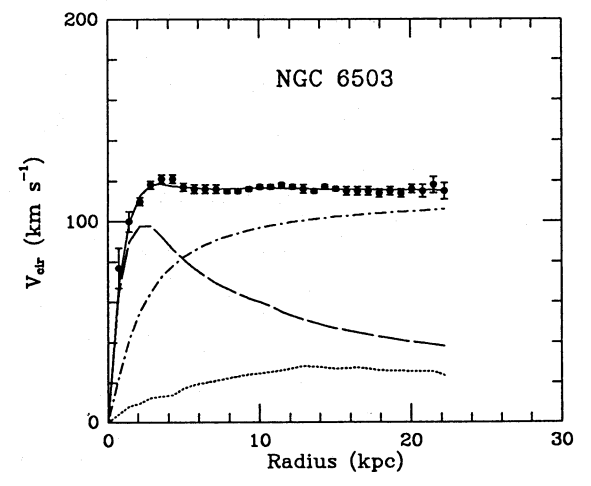
\includegraphics[scale=0.7]{figures/NGC6503_rotcurve.png}
    \caption{Stellar velocity curve fit to NGC 6503 from \cite{Begeman:rot_curves}. Dashed line is the contribution from visible matter. Dotted curves are from gas. Dash-dot curves are from dark matter (DM). Solid line is the composite contribution from all matter and DM sources. Data are indicated with bold dots with error bars. Data agree strongly with a matter + DM composite prediction.}
    \label{fig:gal_rot_curve}
    }
\end{figure}

\Cref{fig:gal_rot_curve} features one of many rotation curves plotted from the stellar velocities within galaxies.
The measured rotation curves mostly feature a flattening of velocities at larder radii which is not expected if the gravity was only coming from luminous matter.
The extension of the flat velocity region also indicates that the DM is distributed far from the center of the galaxy.
Modern velocity measurements include significantly larger objects, galactic clusters, and smaller objects, dwarf galaxies.
Yet, measurements along this regime are leveraging the Virial theorem with Newtonian potential energies.
However, we know Newtonian gravity is not a comprehensive description of gravity.
New observational techniques have been developed since 1978, and those are discussed in the following sections.

%$$$$$$$$$$$$$$$$$$$$$$$$$$$$$$$$$$$$$$$$$$$$$$$$$$$$$$$$$$$$$$$$$$$$$$$$$$$$$$$$$$$%
\subsection{Evidence for Dark Matter: Gravitational Lensing\label{sec:ev4dm_lens}}
%$$$$$$$$$$$$$$$$$$$$$$$$$$$$$$$$$$$$$$$$$$$$$$$$$$$$$$$$$$$$$$$$$$$$$$$$$$$$$$$$$$$%

Modern evidence for dark matter comes from new avenues beyond stellar velocities.
Gravitational lensing from DM is one of these channels from general relativity.
General relativity predicts aberrations in light caused by massive objects.
In recent decades we have been able to measure the lensing effects from compact objects and DM halos.
\Cref{fig:grav_lensing_explained} shows how different massive objects change the final image of a faraway galaxy resulting from gravitational lensing.

\begin{figure}[h!]
    \centering{
        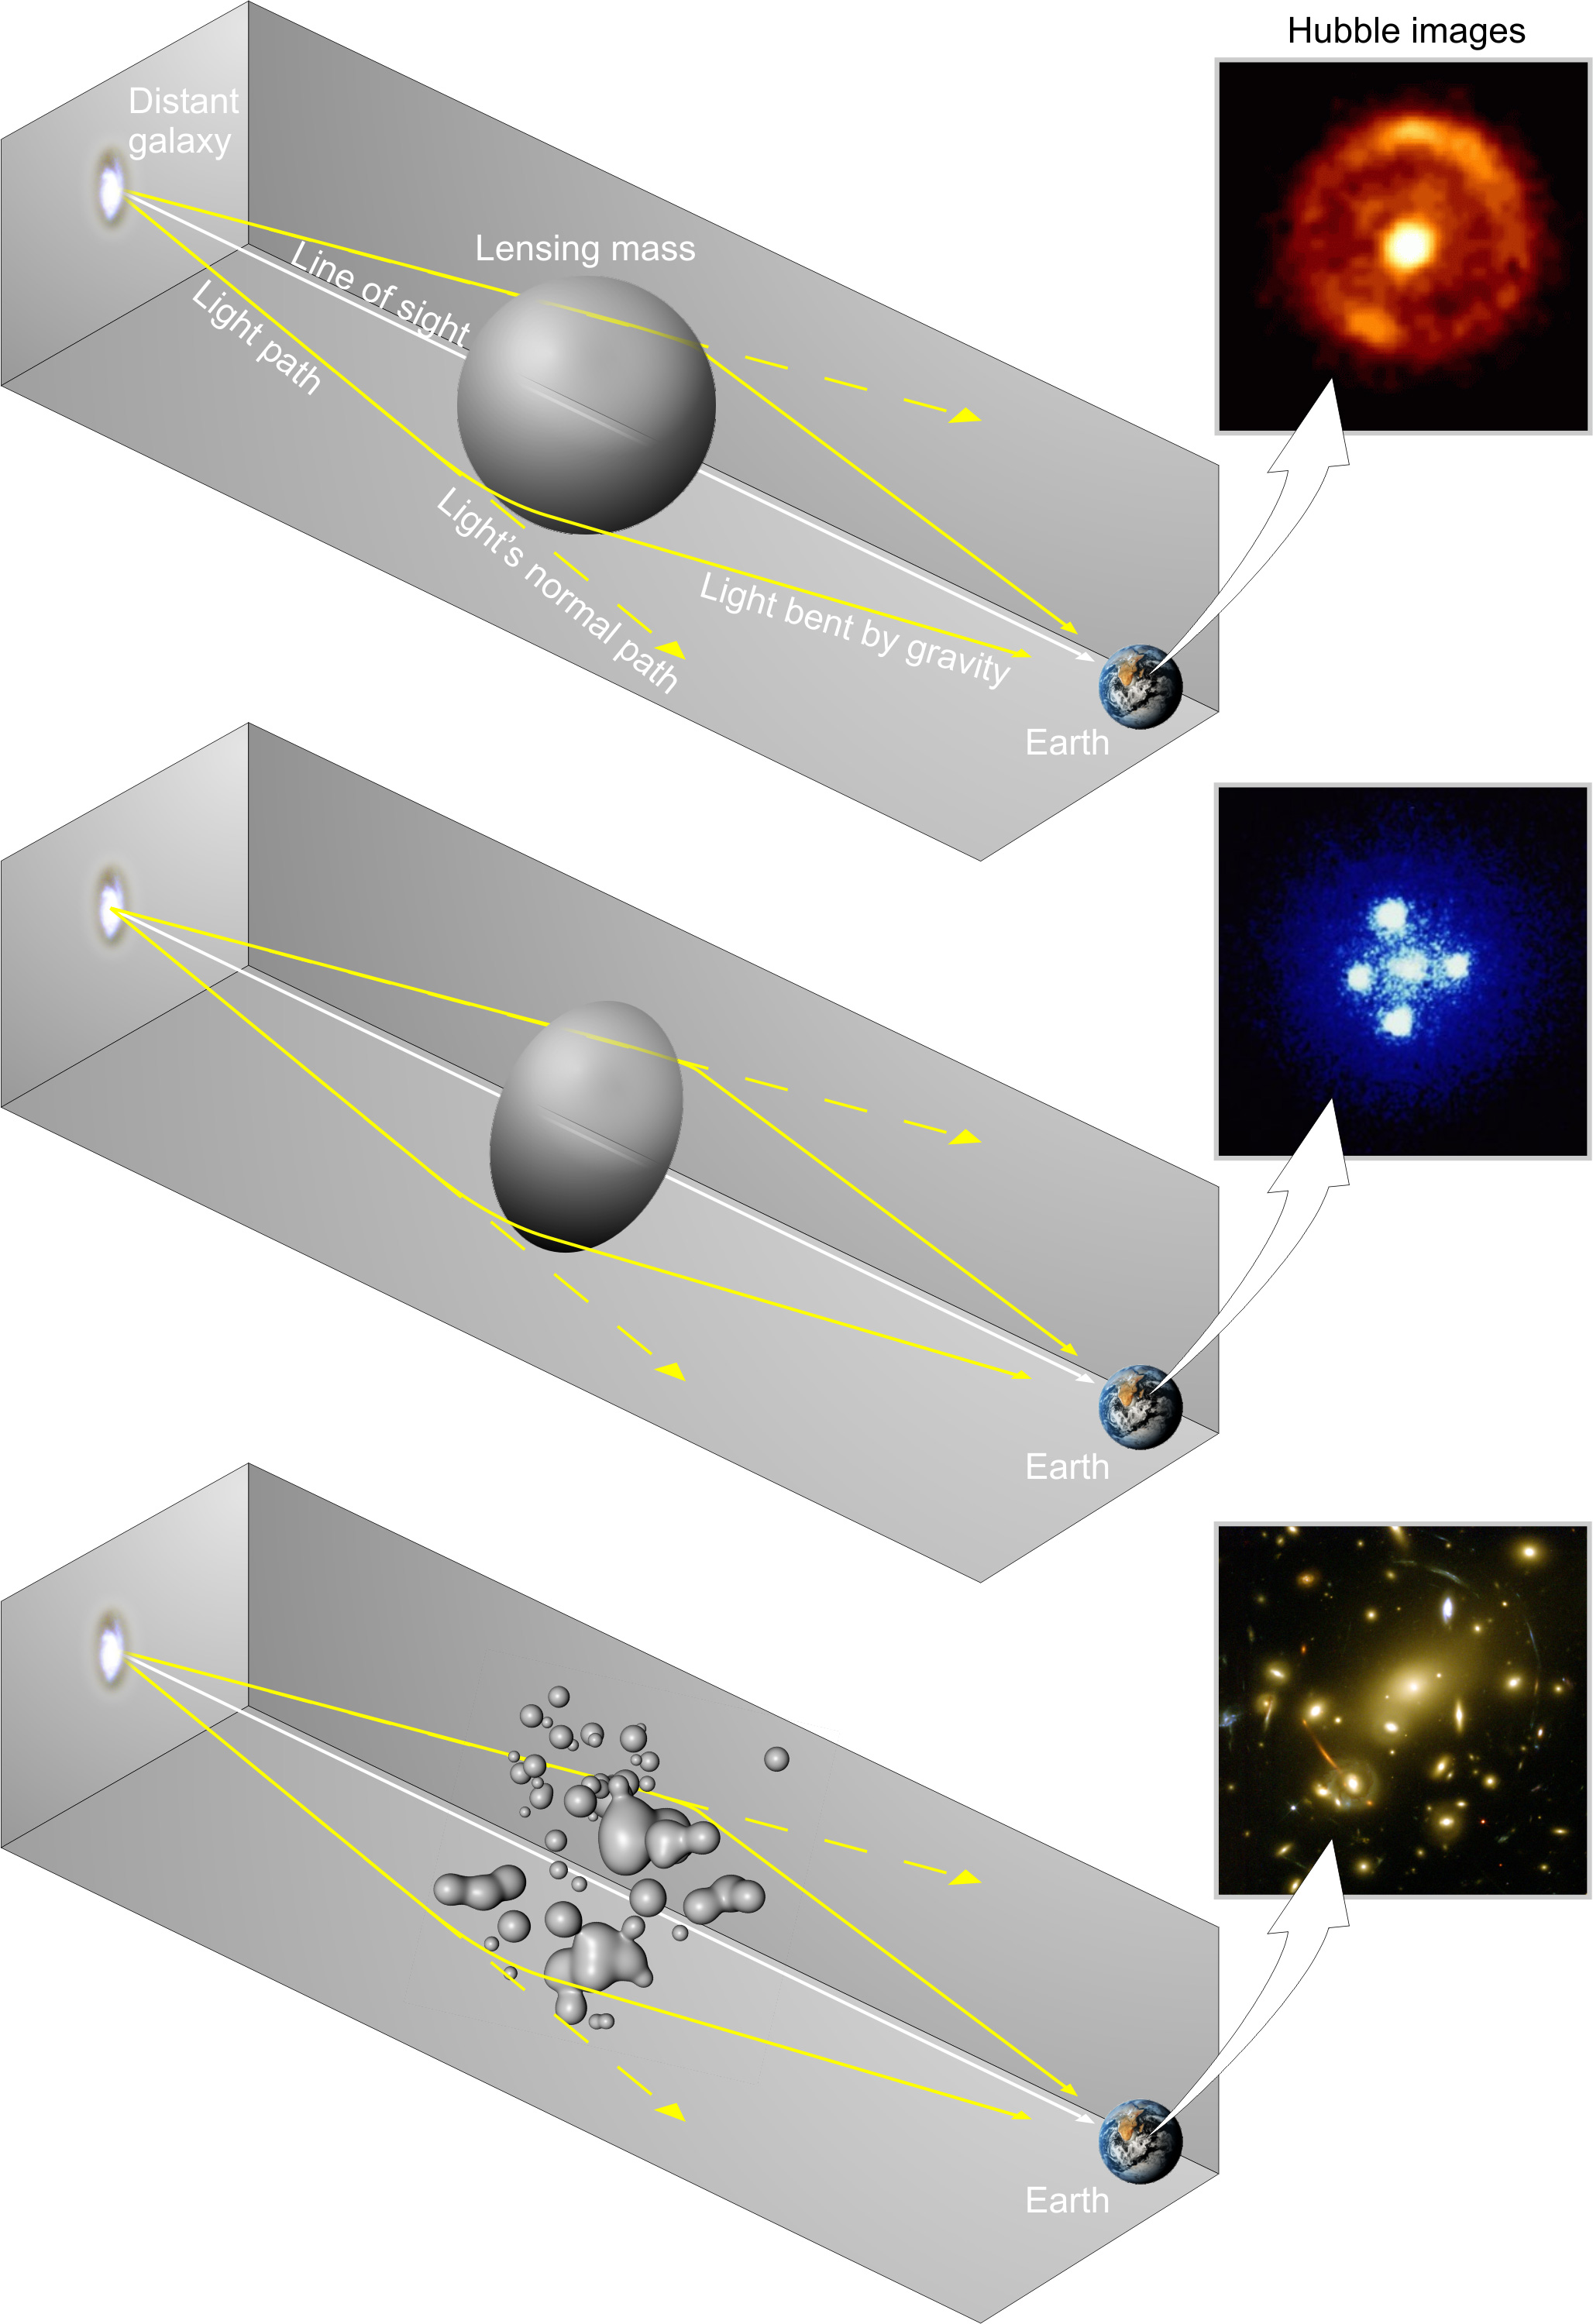
\includegraphics[scale=0.19]{figures/heic0404b.jpg}
        \caption{Light from distant galaxy is bent in unique ways depending on the distribution of mass between the galaxy and Earth. Yellow dashed lines indicate where the light would have gone if the matter were not present. Solid yellow is the path the light actually traverses \cite{eas:grav_lensing}.}
        \label{fig:grav_lensing_explained}
    }
\end{figure}

\begin{figure}[ht]
    \centering{
        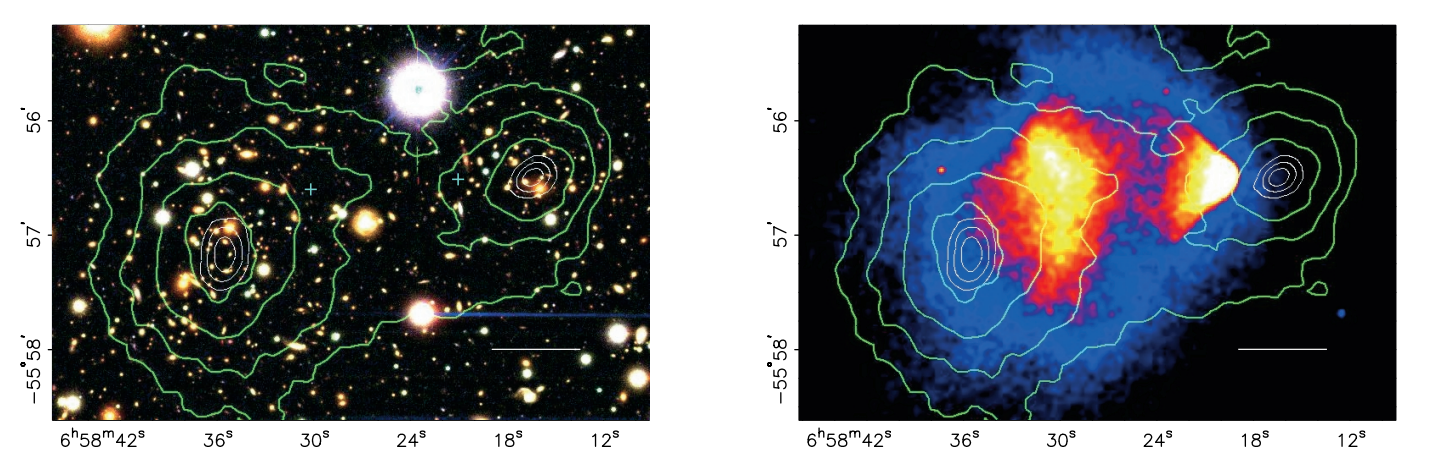
\includegraphics[scale=0.425]{figures/bullet_cluster.png}
        \caption{(left) Optical image of galactic cluster 1E0657-558. (right) X-ray image of the cluster with redder meaning hotter and higher baryon density. (both) Green contours are the reconstructed gravity contours from weak lensing. White rings are the best fit mass maxima at 68.3\%, 95.5\%, and 99.7\% confidence. The matter maxima of the clusters are clearly separated from x-ray maxima. \cite{Clowe:BulletCluster}}
        \label{fig:bullet_cluster}
    }
\end{figure}

Gravitational lensing provides additional compelling evidence for DM.
The observation of two merging galactic clusters in 2006, shown in \Cref{fig:bullet_cluster}, provided a compelling argument for DM outside the Standard Model.
These clusters merged recently in astrophysical time scales.
Galaxies and star cluster have mostly passed by each other as the likelihood of stars colliding within them is low.
Therefore, these massive objects will mostly track the highest mass, dark and/or baryonic, density.
Yet, the intergalactic gas is responsible for the majority of the baryonic mass in the systems \cite{Hooper:DMHistory}.
These gas bodies will not phase through so heat up and compress as they collide together.
The hot gas is located via x-ray emission from the cluster.
Two observations of the clusters were performed independently of each other.

The first was the lensing of light around the galaxies due to their gravitational influences.
When celestial bodies are large enough, the gravity they exert bends space and time itself.
The warped space-time lenses light and will deflect in an analogous way to how glass lenses will bend light, see \Cref{fig:grav_lensing_explained}.
With a sufficient understanding of light sources behind a massive object, we can reconstruct the contours of the gravitational lenses.
The gradient of the contours shown in \Cref{fig:bullet_cluster} then indicates how dense the matter is and where it is.
In the absence of DM, it should also map out where the majority of the mass is.

The x-ray emission is then be observed from the clusters.
Since these galaxies are mostly gas and are merging, the gas should be getting hotter.
If they are merging, the x-ray emissions should be the strongest where the gas is mostly moving through each other.
Hence, X-ray emission maps out where the gas is in the merging galaxy cluster.

The lensing and x-ray observations were done on the Bullet cluster which are featured on \cref{fig:bullet_cluster} \cite{Clowe:BulletCluster}.
The x-ray emissions do not at all align with the gravitational contours.
The incongruence in mass density and baryon density suggests that there is a lot of matter somewhere that does not interact with light.
Moreover, this DM cannot be baryonic \cite{Clowe:BulletCluster}.
The Bullet Cluster measurement did not really tell us what DM is exactly, but it did give the clue that DM also does not interact with itself very strongly.
If DM did interact strongly with itself, then it would have been more aligned with the x-ray emission \cite{Clowe:BulletCluster}.
There have been follow-up studies of galaxy clusters with similar results.
The Bullet Cluster and others like it provide a persuasive case against something possibly amiss in our gravitational theories.

%$$$$$$$$$$$$$$$$$$$$$$$$$$$$$$$$$$$$$$$$$$$$$$$$$$$$$$$$$$$$$$$$$$$$$$$$$$$$$$$$$$$%
\subsection{Evidence for Dark Matter: Cosmic Microwave Background\label{sec:ev4dm_cmb}}
%$$$$$$$$$$$$$$$$$$$$$$$$$$$$$$$$$$$$$$$$$$$$$$$$$$$$$$$$$$$$$$$$$$$$$$$$$$$$$$$$$$$%

\begin{figure}[h]
    \centering{
        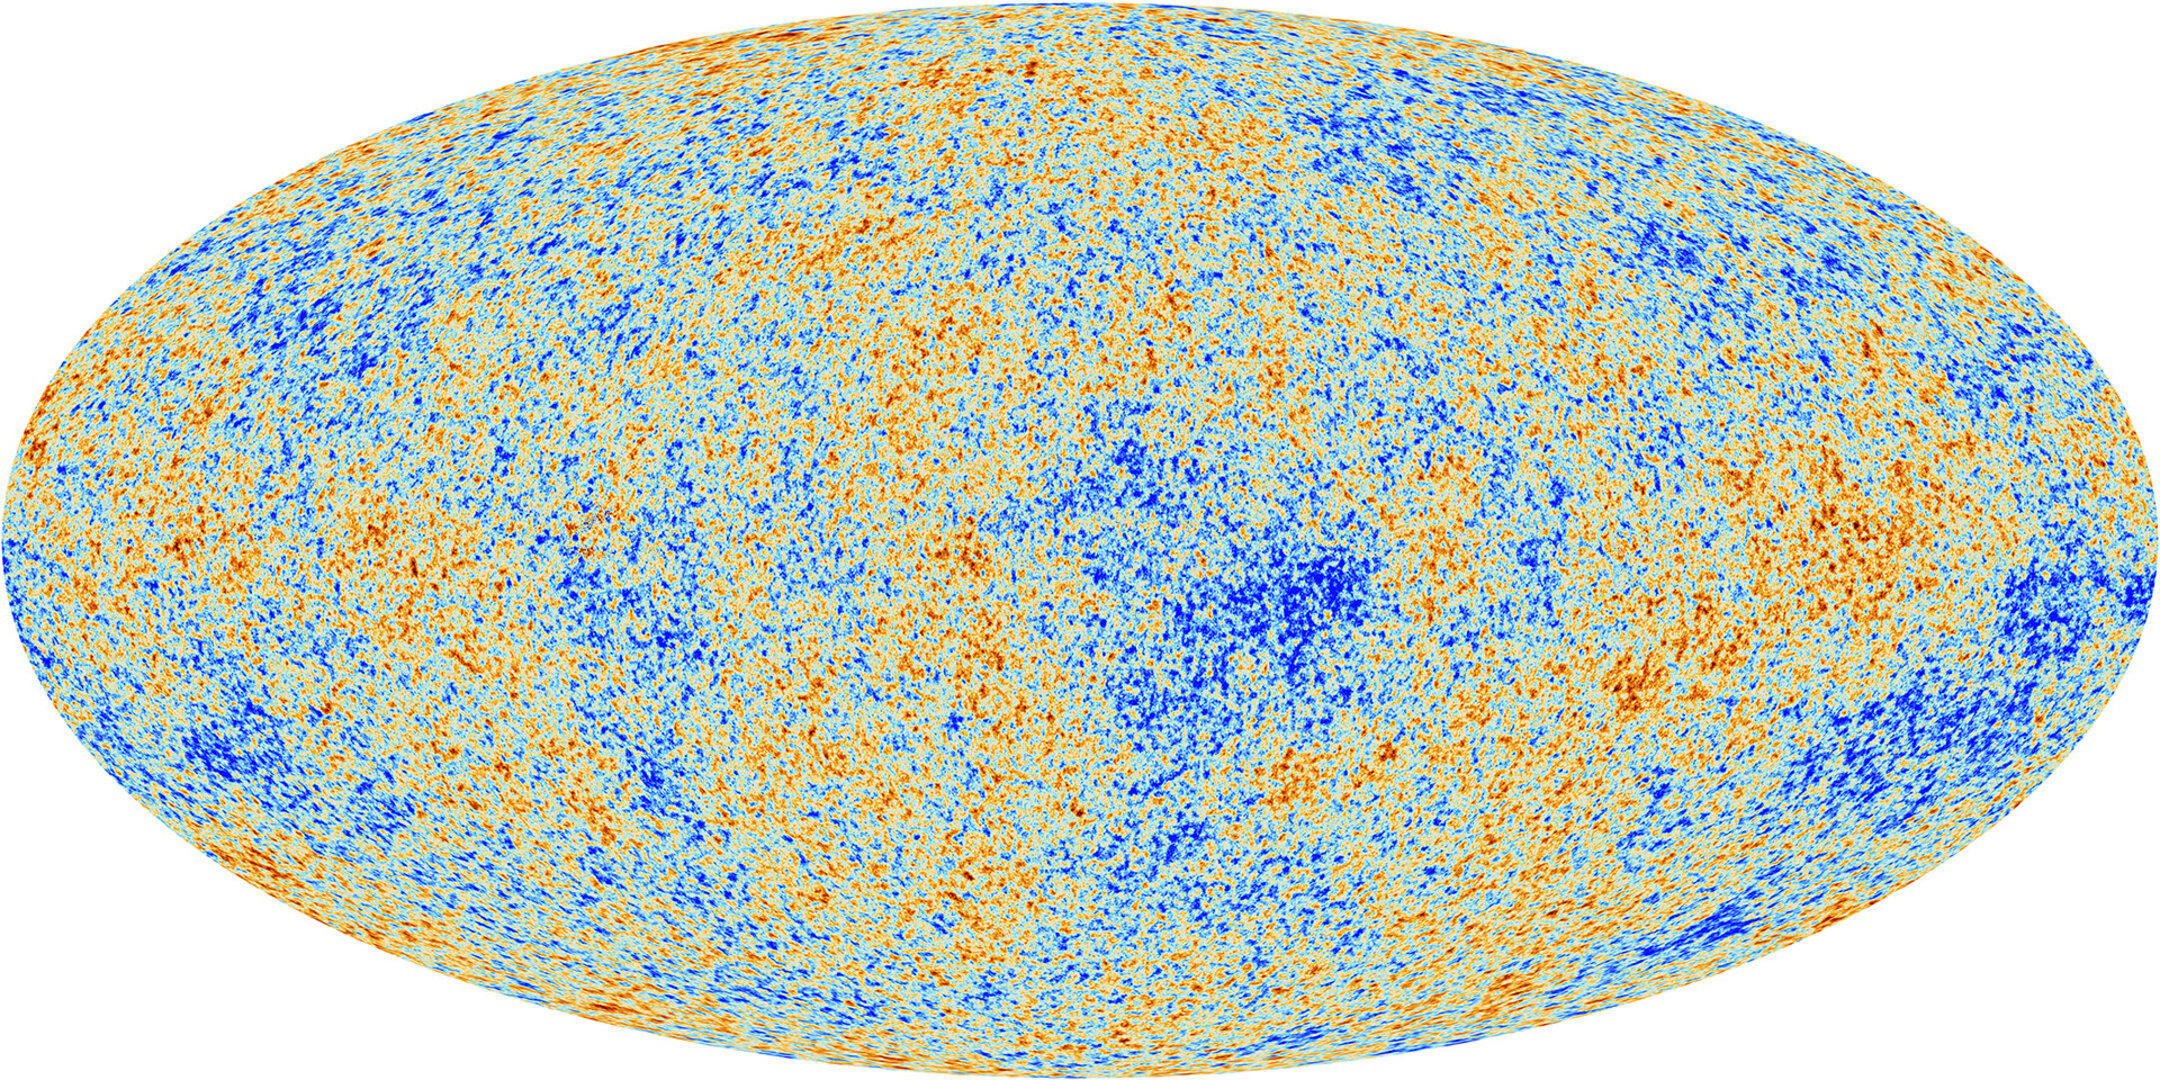
\includegraphics[scale=0.215]{figures/Planck_CMB_pillars.jpg}
        \caption{Plank CMB sky. Sky map features small variations in temperature in primordial light. These anisotropies are used to make inferences about the universe's energy budget and developmental history. \cite{Plank:CMB}}
        \label{fig:CMB}
    }
\end{figure}

The Cosmic Microwave Background (CMB) is the primordial light from the early universe when Hydrogen atoms formed from the combination of free electron and proton soup in the early universe.
Prior to this recombination, the universe was too hot to form atoms and was opaque to light.
The CMB is the earliest light we can observe; released when the universe was about 380,000 years old.
Then we look at how the simulated universes look like compared to what we see.
\Cref{fig:CMB} is the most recent CMB image from the Plank satellite after subtracting the average value and masking the galactic plane \cite{Plank:CMB}.
Redder regions indicate a slightly hotter region in the CMB, and blue indicates colder.
The intensity variations are on the order of 1 in 1000 with respect to the average value.

\begin{figure}[ht]
    \centering{
        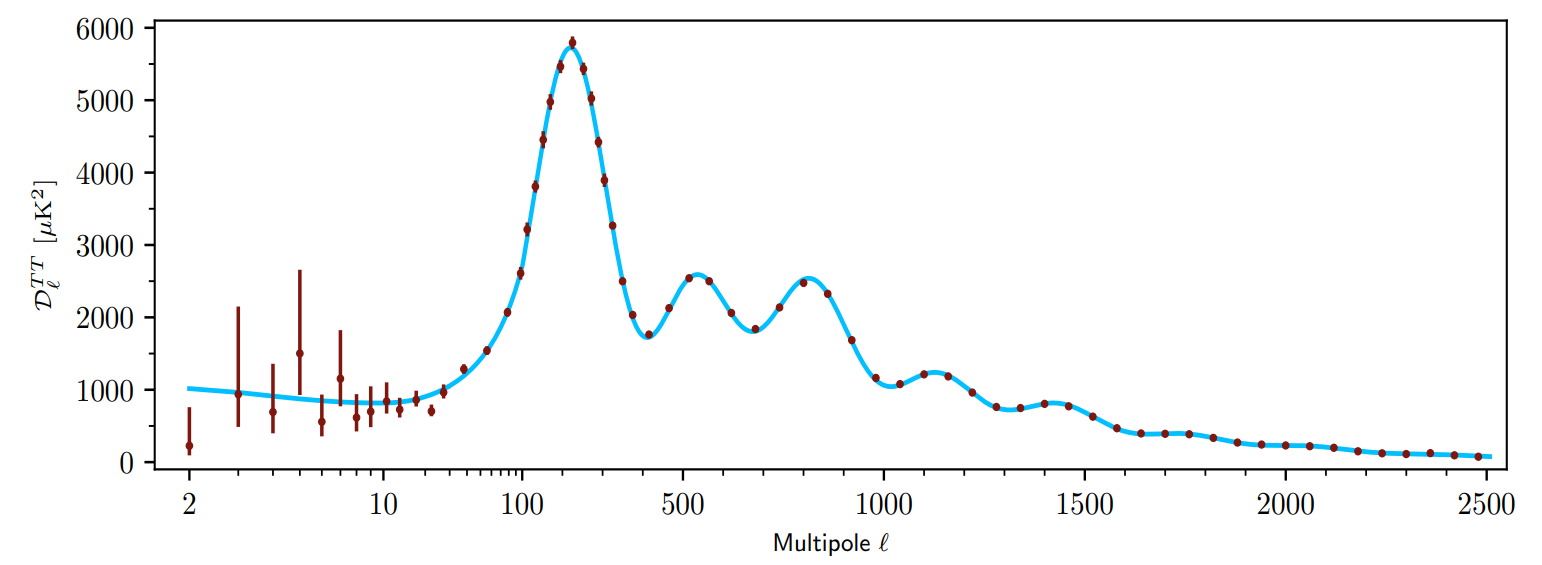
\includegraphics[scale=0.4]{figures/multipole.png}
        \caption{Observed Cosmic Microwave Background power spectrum as a function of multipole moment from Plank observatory \cite{Plank:CMB}. Blue line is the best fit model from \lcdm. Red points and lines are data and error, respectively. }
        \label{fig:multipole}
    }
\end{figure}

The Cosmic Microwave Background shows that the universe had DM in it from an incredibly early stage.
To measure the DM, Dark Energy, and matter fractions of the universe from the CMB, the image is analyzed into a power spectrum, which shows the amplitude of the fluctuations as a function of spherical multipole moments.
\lcdm~provides the best fit to the power spectra of the CMB as shown in \cref{fig:multipole}.
The CMB power spectrum is quite sensitive to the fraction of each energy contribution in the early universe.
Low \textit{l} modes are dominated by variations in gravitational potential.
Intermediate \textit{l} emerge from oscillations in the photon-baryon fluid from competing baryon pressures and gravity.
High \textit{l} is a damped region from the diffusion of photons during electron-proton recombination. \cite{Greene:cosmology_dm}

\begin{figure}[ht]
    \centering{
        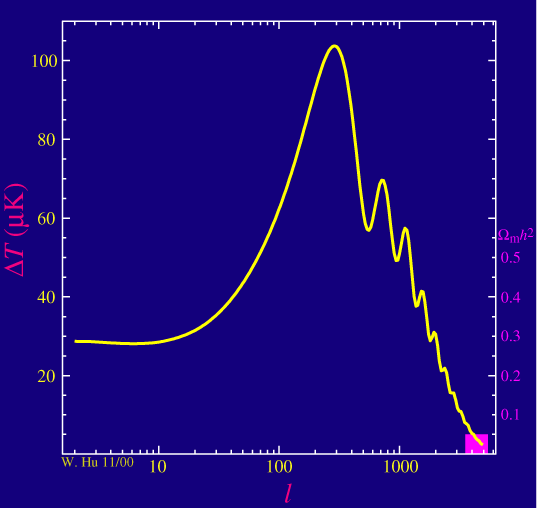
\includegraphics[scale=0.285]{figures/LCDM_multipole/frame_00_delay-0.2s.png}\hfill
        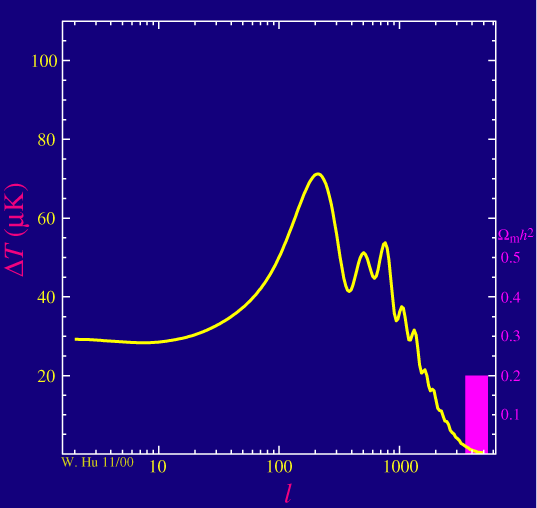
\includegraphics[scale=0.285]{figures/LCDM_multipole/frame_06_delay-0.2s.png}\hfill
        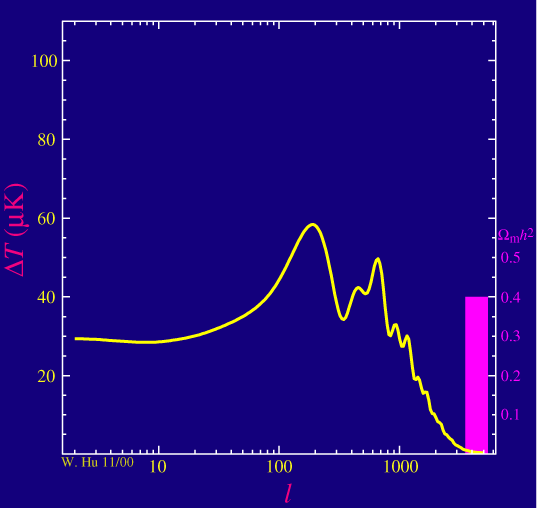
\includegraphics[scale=0.285]{figures/LCDM_multipole/frame_16_delay-0.2s.png}
        \caption{Predicted power spectra of CMB for different $\Omega_m h^2$ values for fixed baryon density from \cite{waynehu:dm_anim}. (left) Low $\Omega_m h^2$ increases the prominence of first and second peaks. (middle) $\Omega_m h^2$ is most similar to the observed power spectrum. The second and third peaks are similar in height. (right) $\Omega_mh^2$ is large which suppresses the first peak and raises the prominence of the third peak.}
        \label{fig:CMB_vibratemodes}
    }
\end{figure}

The harmonics would look quite different for a universe with less DM.
\Cref{fig:CMB_vibratemodes} demonstrates the effect $\Omega_m h^2$, the mass fraction, has on the expected power spectrum for fixed baryon matter density. \cite{waynehu:dm_anim}
Sweeping  $\Omega_m h^2$ while keeping the baryon mass fraction fixed clearly shows the effect dark matter has on the CMB power spectrum.
The observations fit well with the \lcdm~model, and the derived fractions are as follows.
The matter fraction: $\Omega_m = 0.3153$; and the baryon fraction: $\Omega_b = 0.04936$ \cite{Plank:CMB}.
Plank's observations also provide a measure of the Hubble constant, $H_0$.
$H_0$ especially has seen a growing tension in the past decade that continues to deepened with observations from instruments like the James Webb Telescope \cite{JWST:hubble_tension,Freedman:hubble_tension}.
As Hubble tensions deepen, we may find that perhaps \lcdm, despite its successes, is missing some critical physics.

Overall, the Newtonian motion of stars in galaxies, weak lensing from galactic clusters, and power spectra from primordial light form a compelling body of research in favor of dark matter.
It takes another leap of theory and experimentation to make observations of DM that are non-gravitational in nature.
In \cref{sec:evidence4dm}, the evidence for DM implies strongly that the DM is matter and not a lost parameter in the gravitational fields between massive objects.
Finally, if we take one axiom: that this matter has quantum behavior, such as being described by some Bohr wavelength and abiding by some fermion or boson statistics; then we arrive at particle dark matter.
One particle DM hypothesis is the Weakly Interacting Massive Particle (WIMP).
This DM candidate theory is discussed further in the next section and is the focus of this thesis.

%-----------------------------------------------------------------------------------%
\section{Searching for Dark Matter: Particle DM}\label{sec:dm_search}
%-----------------------------------------------------------------------------------%

\begin{figure}[h]
    \centering{
        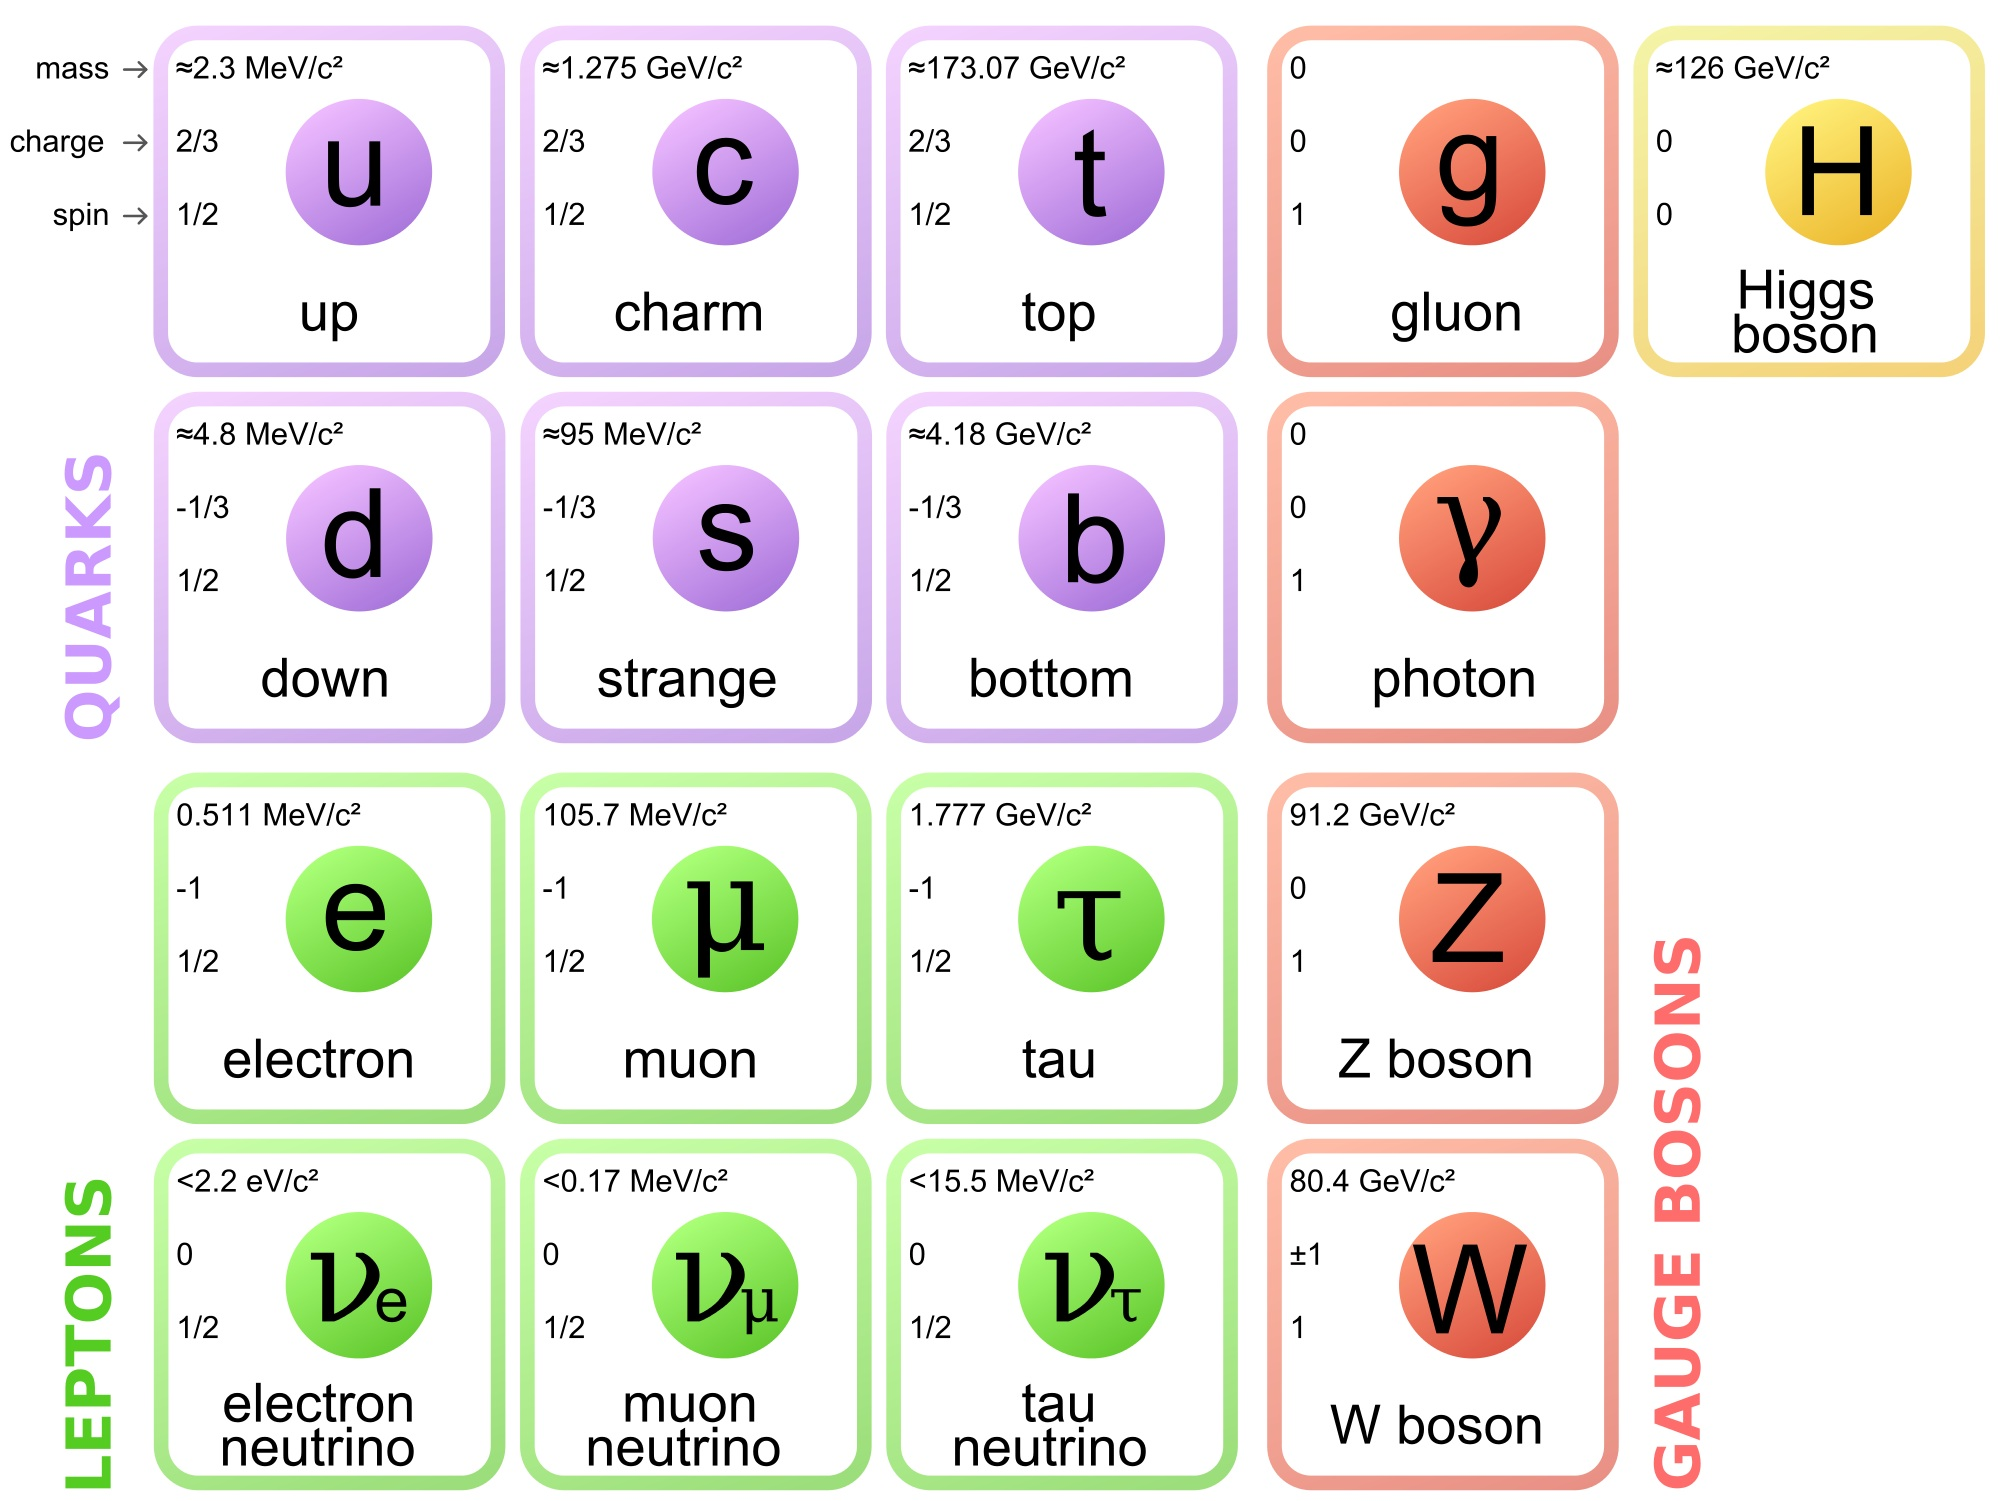
\includegraphics[scale=0.225]{figures/SM.jpg}
    }
    \caption{The Standard Model (SM) of particle physics. Figure taken from \cite{sm_table}}
    \label{fig:SM}
\end{figure}

\Cref{fig:SM} shows the Standard Model of particle physics and is currently the most accurate model for the dynamics of fundamental particles like electrons and photons.
The current status of the SM does not have a viable DM candidate.
When looking at the standard model, we can immediately exclude any charged particle because charged particles interact strongly with light.
Specifically, this will rule out the following charged, fundamental particles: $e,\mu, \tau, W, u, d, s, c, t, b$ and their corresponding antiparticles.
Recalling from \cref{sec:basicDM} that DM must be long-lived and stable over the age of the universe, we exclude all SM particles with decay half-lives at or shorter than the age of the universe.
The lifetime constraint additionally eliminates the $Z$ and $H$ bosons.
Finally, the candidate DM needs to be somewhat massive.
Recall from \Cref{sec:basicDM} that DM is cold or not relativistic through the universe.
This eliminates the remaining SM particles: $\nu_{e, \mu, \tau}, g, \gamma$ as DM candidates.
Because there are no DM candidates within the SM, the DM problem strongly hints to physics beyond the SM (BSM).

%$$$$$$$$$$$$$$$$$$$$$$$$$$$$$$$$$$$$$$$$$$$$$$$$$$$$$$$$$$$$$$$$$$$$$$$$$$$$$$$$$$$%
\subsection{Shake it, Break it, Make it\label{sec:bop_it}}
%$$$$$$$$$$$$$$$$$$$$$$$$$$$$$$$$$$$$$$$$$$$$$$$$$$$$$$$$$$$$$$$$$$$$$$$$$$$$$$$$$$$%

\begin{figure}[h]
    \centering{
        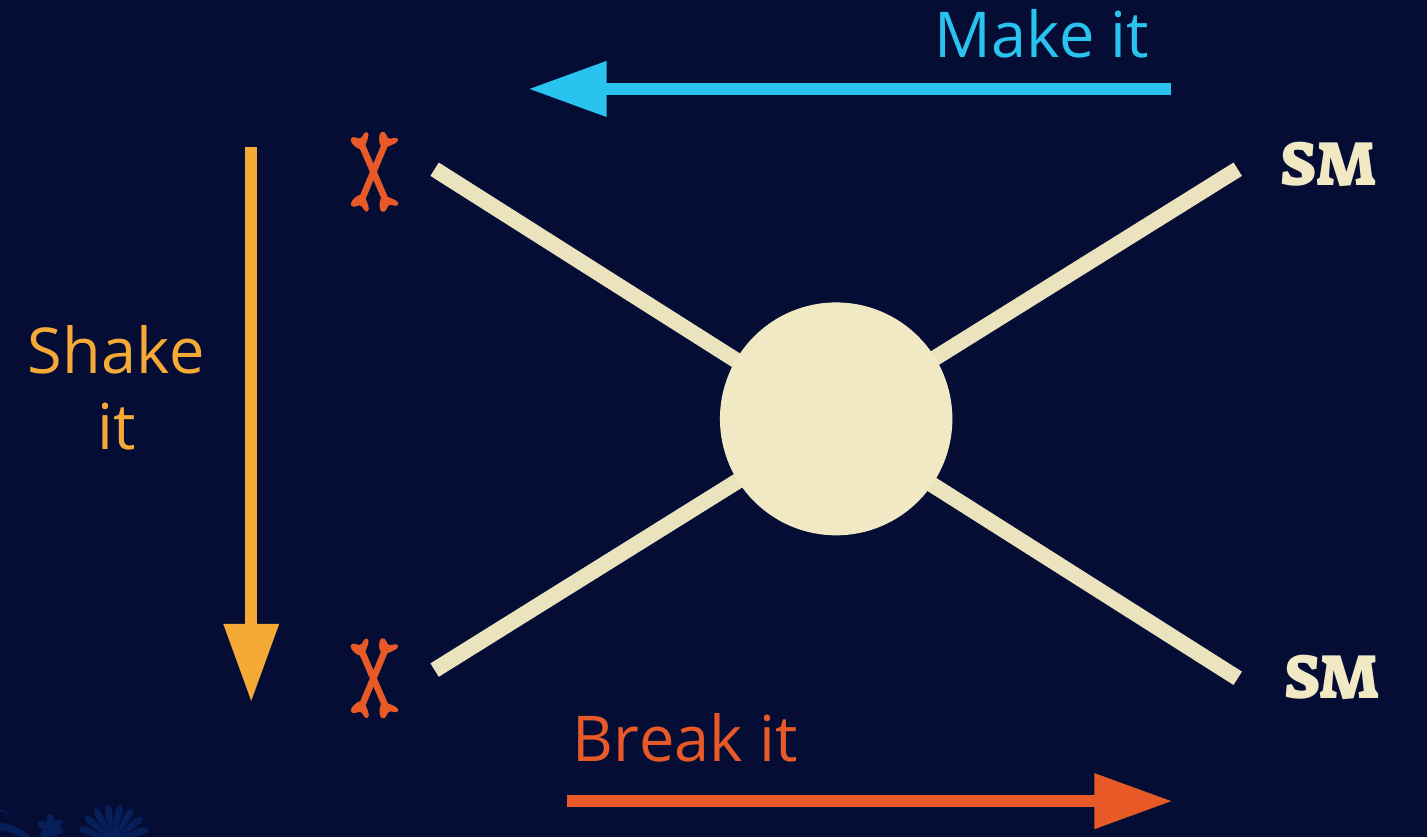
\includegraphics[scale=0.38]{figures/DM_with_SM.png}
        \caption{Simplified Feynman diagram demonstrating the different ways DM can interact with SM particles. The 'X's refer to the DM particles whereas the SM refer to fundamental particles in the SM. The large circle in the center indicates the vertex of interaction and is purposely left vague. The colored arrows refer to different directions of time as well as their respective labels.}
        \label{fig:break_it}
    }
\end{figure}

When considering DM that couples in some way with the SM, the interactions are roughly demonstrated by interaction demonstrated in \Cref{fig:break_it}.
The figure is a simplified Feynman diagram where the arrow of time represents the interaction modes of: \textbf{Shake it, Break it, Make it}.

\textbf{Shake it} refers to the direct detection of dark matter.
Direct detection interactions start with a free DM particle and an SM particle.
The DM and SM interact via elastic or inelastic collision and recoil away from each other.
The DM remains in the dark sector and imparts some momentum onto the SM particle.
The hope is that the momentum imparted onto the SM particle is sufficiently high enough to pick up with extremely sensitive instruments.
Because we cannot create the DM in the lab, a direct detection experiment must wait until DM is incident on the detector.
Most direct detection experiments are therefore placed in low-background environments with inert detection media like the noble gas, Xenon. \cite{Cooley:dd_dm}

\textbf{Make it} refers to the production of DM from SM initial states.
The experiment starts with particles in the SM.
These SM particles are accelerated to incredibly high energies and then collide with each other.
In the confluence of energy, DM hopefully emerges as a byproduct of the SM annihilation.
Often it is the collider experiments that are energetic enough to hypothetically produce DM.
These experiments include the world-wide collaborations, ATLAS and CMS at CERN, where protons collide together at extreme energies.
The DM searches, however, are complex.
DM likely does not interact with the detectors and lives long enough to escape the detection apparatus of CERN's colliders.
This means any DM production experiment searches for an excess of events with missing momentum or energy in the events.
An example event with missing transverse momentum is shown in \Cref{fig:met_atlas}.
The missing momentum with no particle tracks implies a weakly interacting particle carried the energy out of the detector.
However, there are other neutral particles in the SM, like neutrons or neutrinos, so any analysis has to account for SM signatures of missing momentum. \cite{atlas:met_dm_precise}

\begin{figure}[h]
    \centering{
        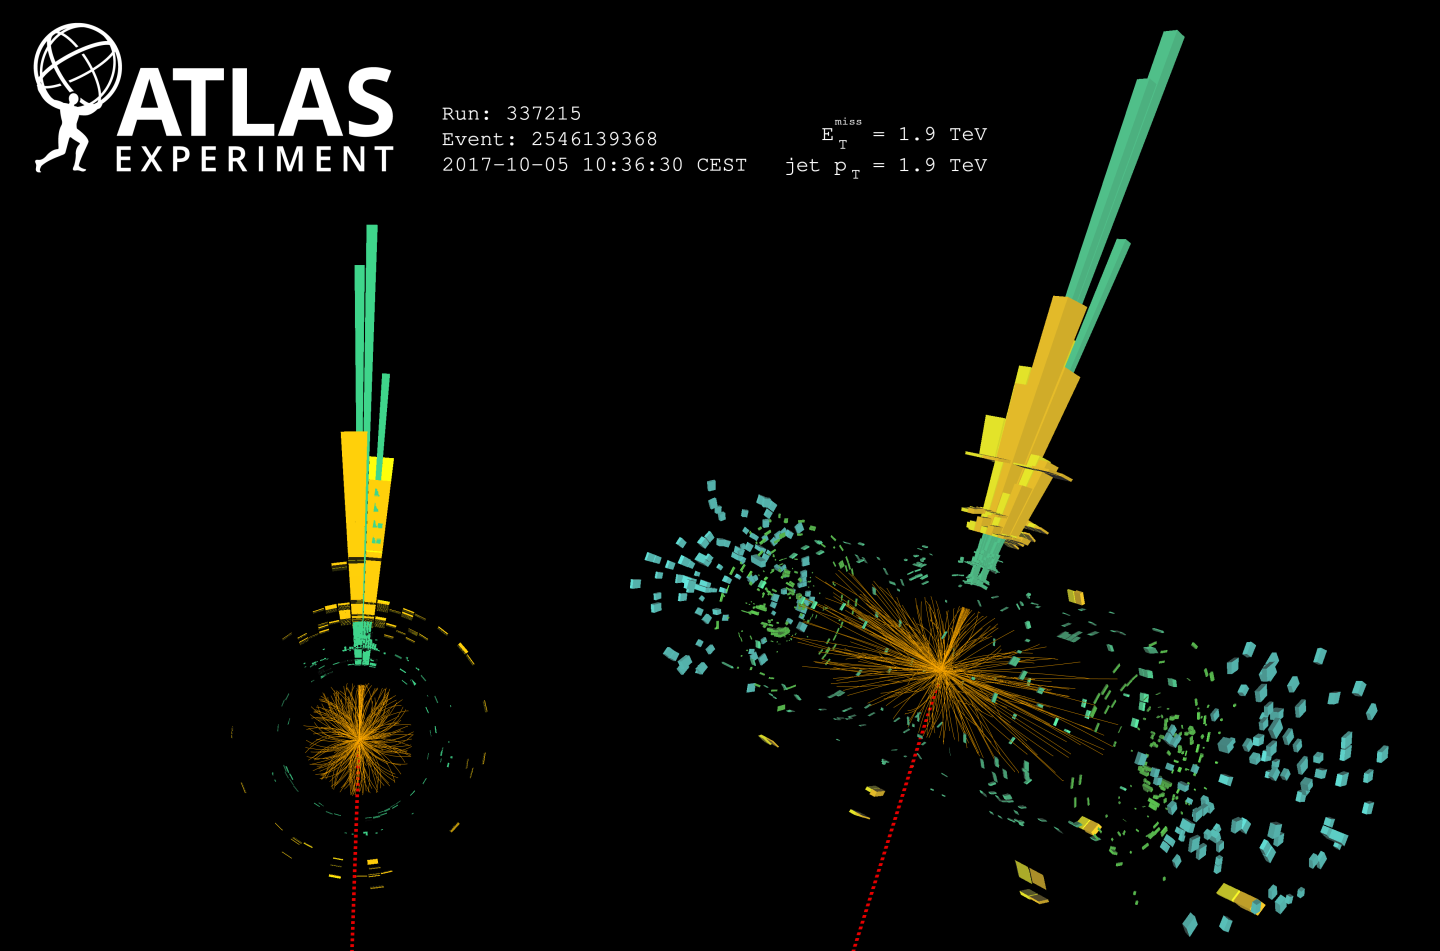
\includegraphics[scale=0.435]{figures/MET_ATLAS.png}
        \caption{A single jet event in the ATLAS detector from 2017 \cite{atlas:dm_precise}. Total transverse momentum was observed to be 1.9 TeV where it should be 0. Missing transverse momentum is inferred to be opposite the observed transverse momentum in order to preserve overall momentum in the event.}
        \label{fig:met_atlas}
    }
\end{figure}

%$$$$$$$$$$$$$$$$$$$$$$$$$$$$$$$$$$$$$$$$$$$$$$$$$$$$$$$$$$$$$$$$$$$$$$$$$$$$$$$$$$$%
\subsection{Break it: Standard Model Signatures of Dark Matter through Indirect Searches\label{sec:break_it}}
%$$$$$$$$$$$$$$$$$$$$$$$$$$$$$$$$$$$$$$$$$$$$$$$$$$$$$$$$$$$$$$$$$$$$$$$$$$$$$$$$$$$%

\textbf{Break it} refers to the creation of SM particles from the dark sector, and it is the primary focus of this thesis.
The interaction begins with DM in the dark sector.
The hypothesis is that this DM will either annihilate with itself or decay and produce an SM byproduct.
This method is often referred to as the Indirect Detection of DM because we have no lab to directly control or manipulate the DM.
Therefore, most indirect DM searches are performed using observations of known DM densities among astrophysical sources.
The strength is that we have the whole of the universe and its 13.6-billion-year lifespan to use as a detector and particle accelerator.
Additionally, locations of dark matter are well cataloged since it was astrophysical observations that presented the problem of DM in the first place.

\begin{figure}[ht]
    \centering{
        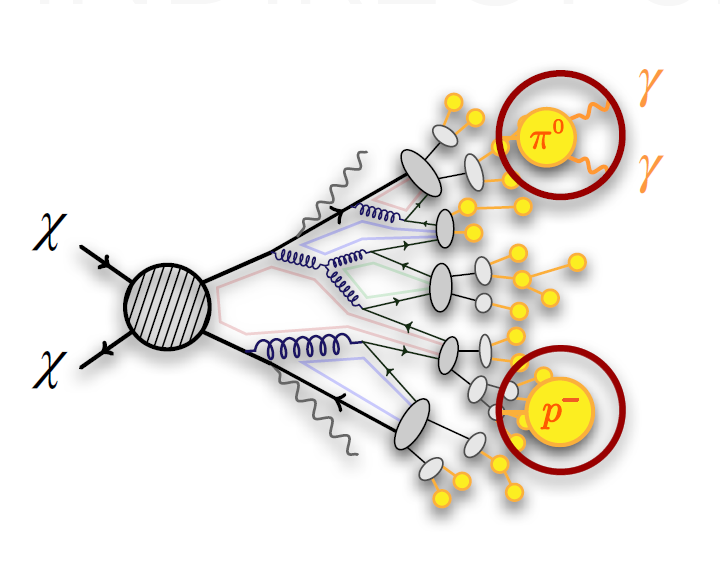
\includegraphics[scale=0.4]{figures/DM_annihilation.png}
        \caption{More detailed pseudo-Feynman diagram of particle cascade from dark matter annihilation into 2 quarks. The quarks hadronize down to stable particles like \textgamma~or the anti-proton ($p^-$). Diagram pulled from ICRC 2021 presentation on DM annihilation search \cite{2021ICRC:glory_duck}.}
        \label{fig:id_dm_ann}
    }
\end{figure}

However, anything can happen in the universe.
There are many difficult to deconvolve backgrounds when searching for DM.
One prominent example is the galactic center.
We know the galactic center has a large DM content because of stellar kinematics in our Milky Way and DM halo simulations.
Yet, any signal from the galactic center is challenging to parse apart from the extreme environment of our supermassive black hole, unresolved sources, and diffuse emission from the interstellar medium \cite{Tracy:les_houches}.
Despite the challenges, any DM model that yields evidence in the other two observation methods, \textbf{Shake it} or \textbf{Make it} must be corroborated with indirect observations of the known DM sources.
Without corroborating evidence, DM observation in the lab is hard-pressed to demonstrate that it is the model contributing to the DM seen at the universal scale.

In the case of WIMP DM, signals are described in terms of primary SM particles produced from DM decay or annihilation.
The SM initial state particles are then simulated down to stable final states such as the $\gamma, \nu, p, \text{or } e$ which can traverse galactic lengths to reach the Earth.

\Cref{fig:id_dm_ann} shows the quagmire of SM particles that emerges from SM initial states that are not stable \cite{2021ICRC:glory_duck}.
There are many SM particles with varying energies that can be produced in such an interaction.
For any arbitrary DM source and stable SM particle, the SM flux from DM annihilating to a neutral particle in the SM, $\phi$, from a region in the sky is described by the following.
\iddmannilationPhi
In \cref{eq:id_dm_flux_phi}, \sv~is the velocity-weighted annihilation cross-section of DM to the SM.
$m_\chi$ refers to the mass of DM, noted with Greek letter $\chi$.
$\frac{dN_{\phi}}{dE_\phi}$ is the N particle flux weighted by the particle energy.
Example spectra are provided in \cref{fig:dm_decay_spectra} for the $\chi\chi \rightarrow$ \parpar{b} $\rightarrow \gamma$ final state.
The integrated terms are performed over the solid angle, $d\Omega$, and line of sight, l.o.s.
$\rho$ is the density of DM for a location $(r, \theta')$ in the sky.
The terms left of the '$\times$' are often referred to as the particle physics component.
The terms on the right are referred to as the astrophysical component.
For decaying DM, the equation changes to\dots
\iddmdecay

In \Cref{eq:id_dm_decay}, $\tau$ is the decay lifetime of the DM.
Just as in \cref{eq:id_dm_flux_phi}, the left and right terms are the particle physics and the astrophysical components respectively.
The integrated astrophysical component of \cref{eq:id_dm_flux} is often called the J-Factor.
Whereas the integrated astrophysical component of \cref{eq:id_dm_decay} is often called the D-Factor.

\begin{figure}[h]
    \centering{
        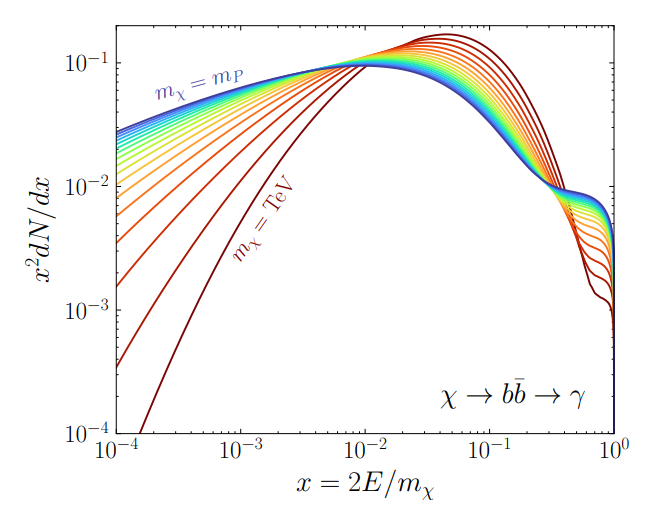
\includegraphics[scale=0.65]{figures/bb_decay_hdm.png}
        \caption{Dark Matter (DM) decay spectrum for $b\bar{b}$ initial state and $\gamma$ final state. Redder spectra are for larger DM masses. Bluer spectra are light DM masses. $x$ is a unitless factor defined as the ratio of the mass of DM, $m_\chi$, and the final state particle energy $E_{\gamma}$. Figure from \cite{Rodd:HDM_spec}.}
        \label{fig:dm_decay_spectra}
    }
\end{figure}

Exact $\chi\chi \rightarrow$ \textbf{SM SM} branching ratios are not known, so it is usually assumed to go 100\% into an SM particle/anti-particle.
Additionally, when a DM annihilation or decay produces one of the neutral, long-lived SM particles ($\nu$ or $\gamma$), the particle can be traced back to a DM source.
For DM above GeV energies, there are very few SM processes that can produce particles with such a high energy.
Seeing such a signal would almost certainly be an indication of the presence of dark matter.
Fortunately, the universe  provides us with the largest volume and lifetime ever for a particle physics experiment.

%-----------------------------------------------------------------------------------%
\section{Sources for Indirect Dark Matter Searches\label{sec:dm_targets}}
%-----------------------------------------------------------------------------------%

\begin{figure}
    \centering{
        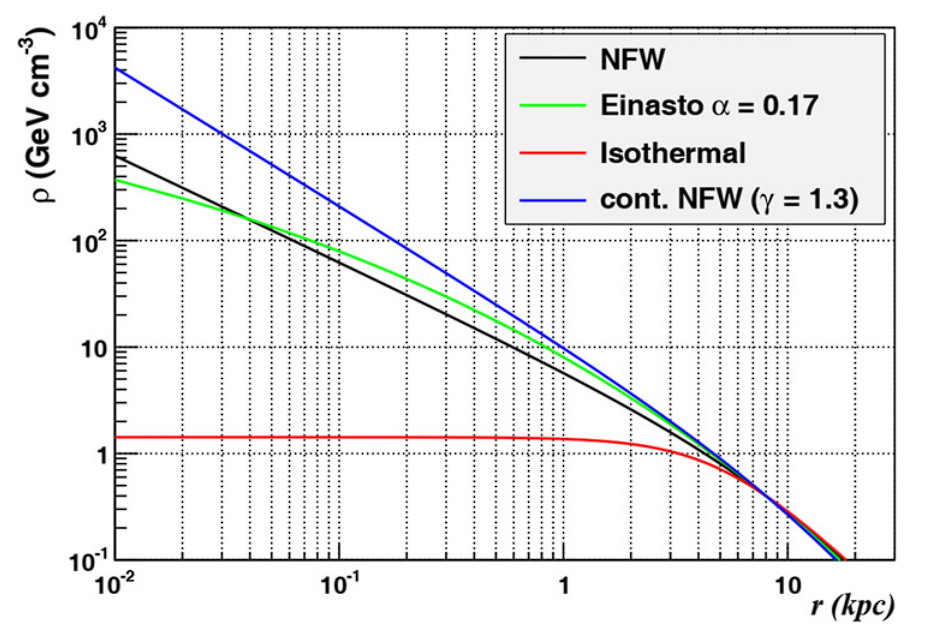
\includegraphics[scale=0.5]{figures/dm_profiles.png}
        \caption{Different dark matter density profiles compared. Some models produce exceptionally large densities at small r \cite{2010:dm_profiles}.}
        \label{fig:dm_profile}
    }
\end{figure}

The first detection of DM relied on optical observations.
Since then, we have developed new techniques to find DM dense regions.
As described in \cref{sec:ev4dm_stars}, many DM dense regions were discovered through observing galactic rotation curves.
Our Milky Way galaxy is among DM dense regions discovered, and it is the largest nearby DM dense region to look at.
Additionally, the DM halo surrounding the Milky Way is clumpy \cite{Tracy:les_houches}.
There are regions in the DM halo of the Milky Way that have more DM than others that have captured gas over time.
These sub-halos were dense enough collapse gas and form stars.
These apparent sub galaxies are known as dwarf spheroidal galaxies (dSphs) and are the main sources studied in this thesis.
Each source type comes with different trade-offs.
Galactic Center studies will be very sensitive to the assumed distribution of DM.
The central DM density can vary substantially as demonstrated in \cref{fig:dm_profile}.
At distances close to the center of the galaxy, or small \textit{r}, the differences in DM densities can be 3-4 orders of magnitude.
Searches toward the galactic center will therefore be quite sensitive to the assumed DM distribution.

Searches dSphs suffer from uncertainties in the DM density less than the galactic center studies.
This is mostly from their diminutive size being smaller than the angular resolution of most high energy astrophysical observatories \cite{Tracy:les_houches}.
The DM content of dSphs are typically determined with the Virial theorem, \cref{eq:virialtheorem}, and are usually majority DM \cite{Tracy:les_houches} in mass.
DSph's tend to be ideal sources to look at for DM searches.
Their environments are quiet with little astrophysical background.
Unlike the galactic center, the most energetic components of dSph's are the stars within them versus a violent accretion disc around a black hole.
All this together means that dSph's are among the best sources to look at for indirect DM searches.
dSph's are the targets of focus for this thesis.

%-----------------------------------------------------------------------------------%
\section{Multi-Messenger Dark Matter \label{sec:mult-messengerDM}}
%-----------------------------------------------------------------------------------%

Astrophysics entered a new phase in the past few decades that leverages our increasing sensitivity to SM channels and general relativity (GR).
Up until the 21st century, astrophysical observations were performed with photons ($\gamma$) only.
Astrophysics with this 'messenger' is fairly mature now.
Novel observations of the universe have since only adjusted the sensitivity of the wavelength of light that is observed except at MeV energies.
Gems like the CMB \cite{Plank:CMB}, and more have ultimately been observations of different wavelengths of light.
Multi-messenger astrophysics proposes using other SM particles such the $p^{+/-},  \nu$, or gravitation waves predicted by general relativity.

The experiment LIGO had a revolutionary discovery in 2016 with the first detection of a binary black hole merger \cite{2016:grav_waves}.
This opened the collective imagination to observing the universe through gravitational waves.
There has also been a surge of interest in the neutrino ($\nu$) sector.
IceCube demonstrated that we are sensitive to neutrinos in regions that correlate with significant photon emission like the galactic plane \cite{2023:IC3_galactic_plane}.
Neutrinos, like gravitational waves and light, travel mostly unimpeded from their source to our observatories.
This makes pointing to the originating source of these messengers much easier than it is for cosmic rays which are deflected from their source by magnetic fields.

\begin{figure}[h]
    \centering{
        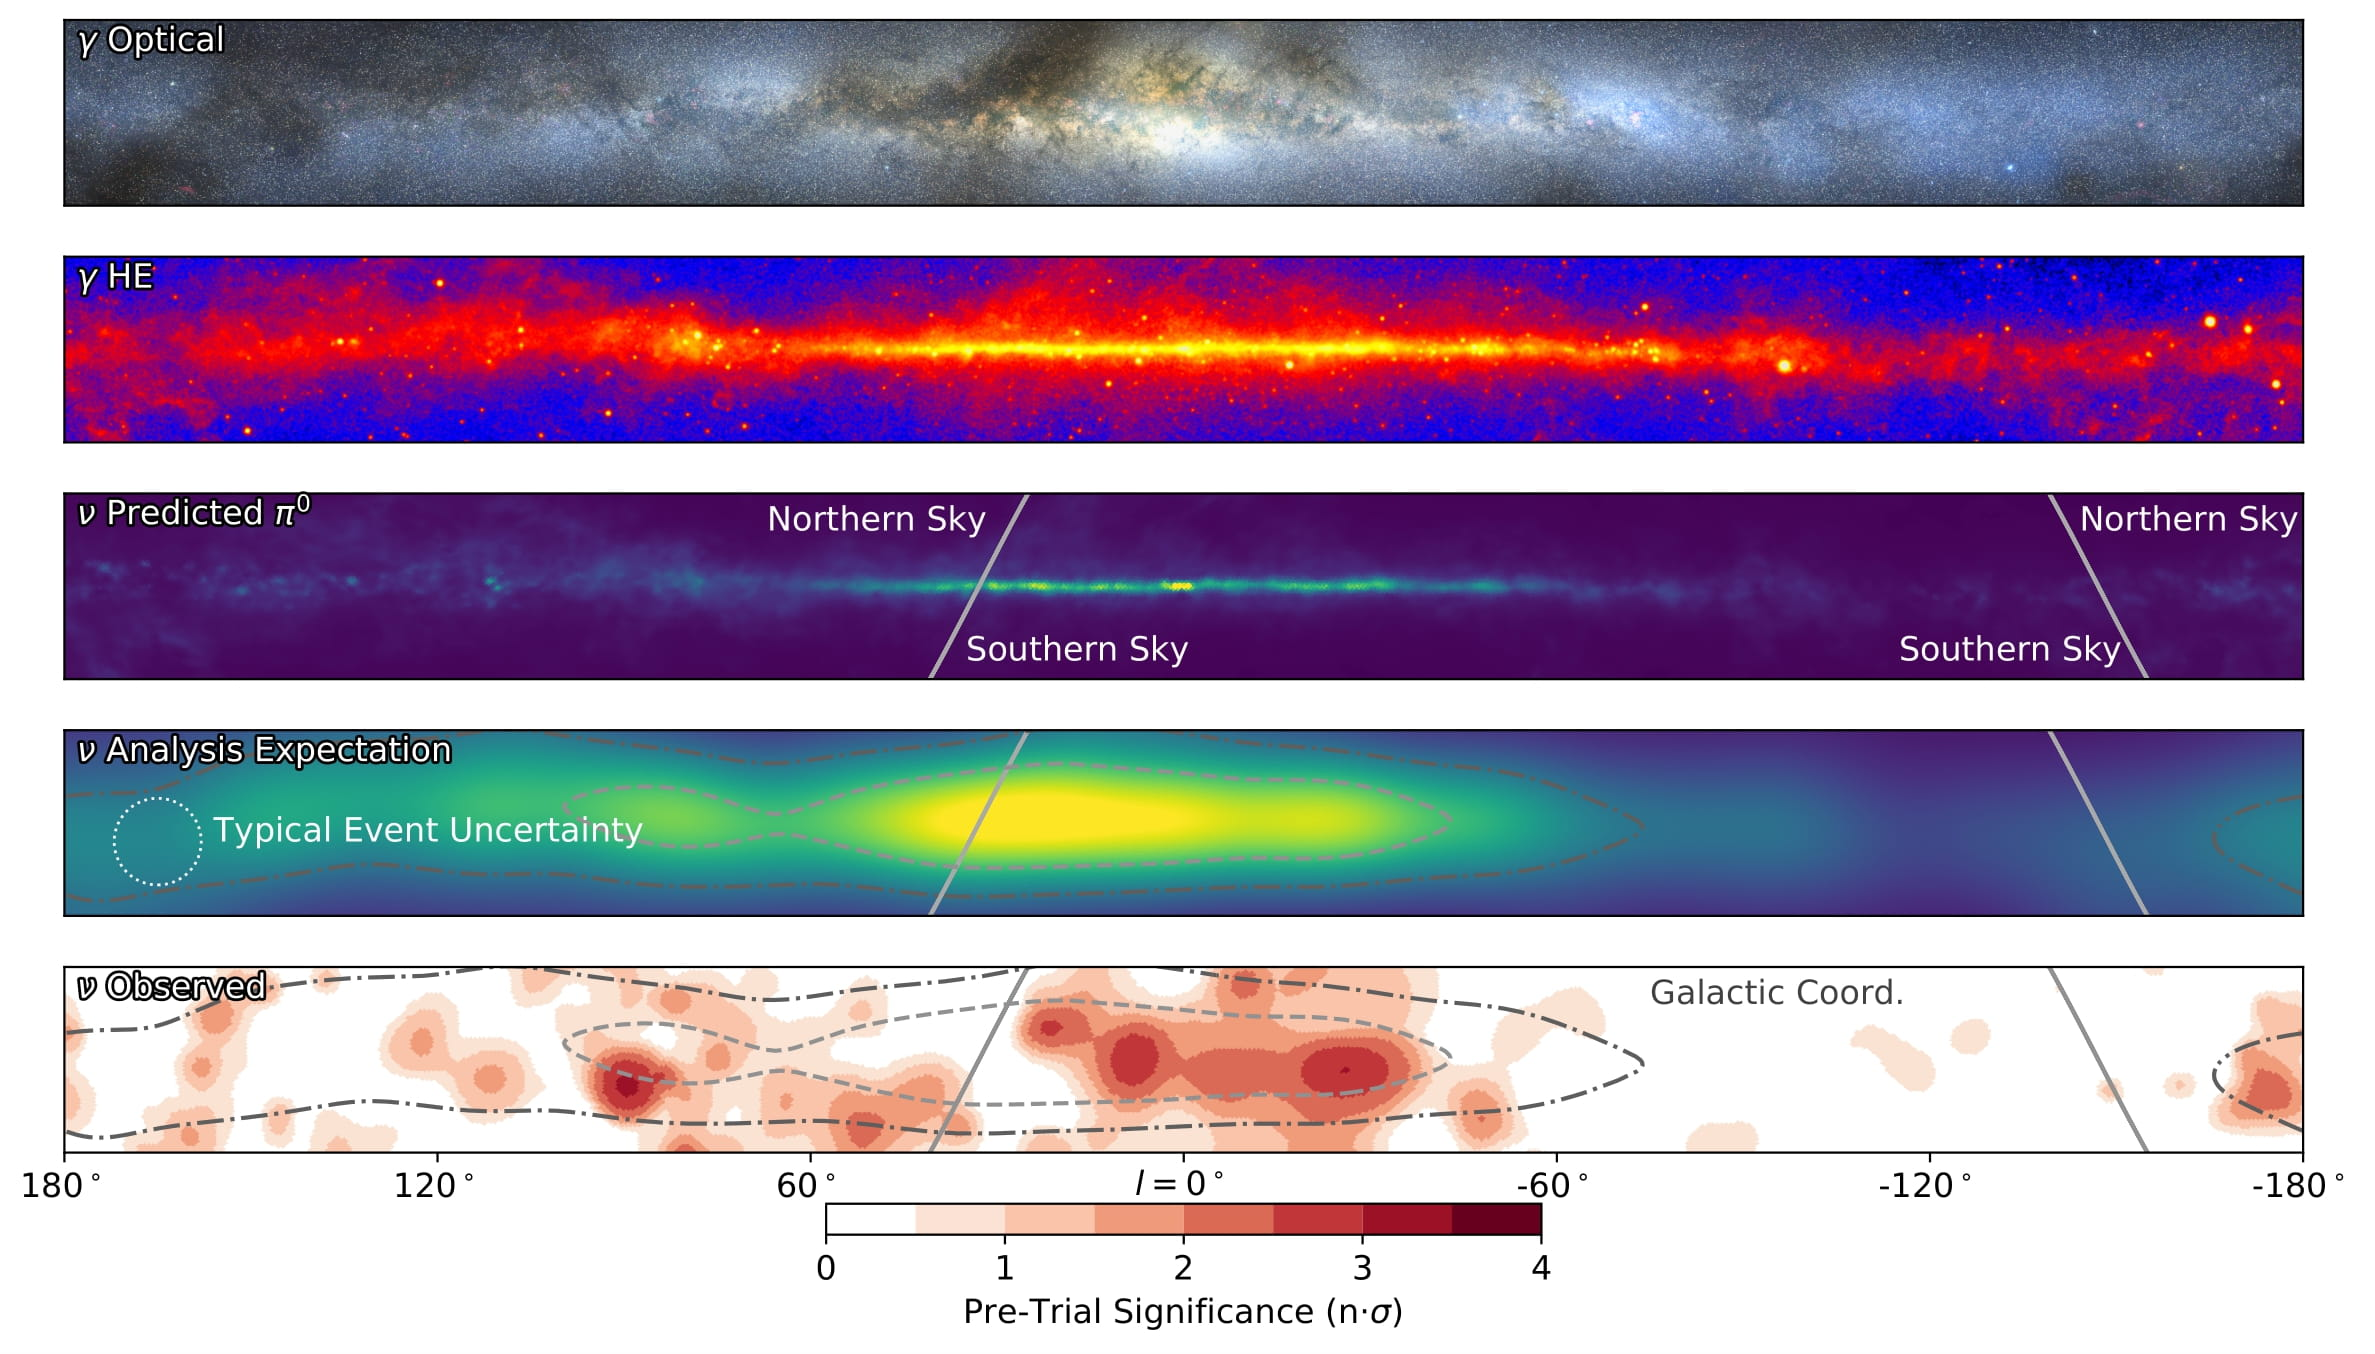
\includegraphics[scale=0.41]{figures/ic3_galacticplane.jpg}
        \caption{The Milky Way Galaxy in photons ($\gamma$) and neutrinos ($\nu$) \cite{2023:IC3_galactic_plane}. The Galactic center is at l = 0\textdegree and is the brightest region in all panels. (top) An Optical color image of the Milky Way galaxy seen from Earth. Clouds of gas and dust obscure some light from stars. (2nd down) Integrated flux of $\gamma$-rays observed by the Fermi-LAT telescope \cite{fermi:mw_plane}. (middle) Expected neutrino emission that corresponds with Fermi-LAT observations. (2nd up) Expected neutrino emission profile after considering detector systematics of IceCube. (bottom) Observed neutrino emission from region of the galactic plane. Substantial neutrino emission was detected.}
        \label{fig:ic3_mw}
    }
\end{figure}

The IceCube collaboration recently published a groundbreaking result of the Milky Way in neutrinos.
The recent result from IceCube, shown in \Cref{fig:ic3_mw}, proves that we can make observations under different messenger regimes.
The top two panels show the appearance of the galactic plane to different wavelengths of light.
Some sources are more apparent in some panels, while others are not.
This new channel is powerful because neutrinos are readily able to penetrate through gas and dust in the Milky Way.
This new image also refines our understanding of how high energy particles are produced.
For example, the fit to IceCube data prefers neutrino production from the decay of $\pi^0$ \cite{2023:IC3_galactic_plane}.

\begin{figure}[h]
    \centering{
        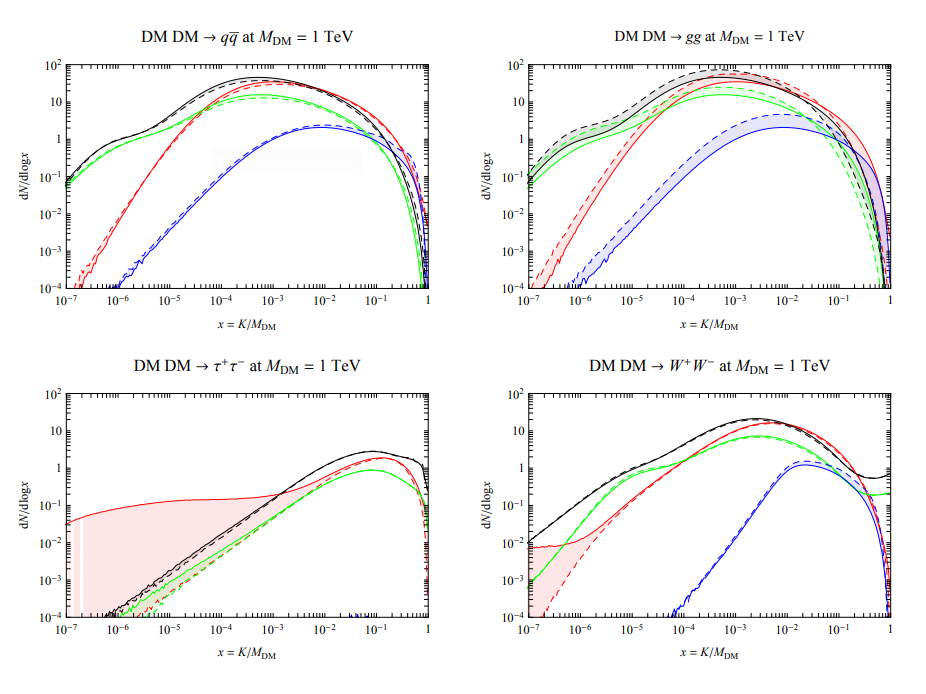
\includegraphics[scale=0.65]{figures/pppc_spectra.png}
        \caption{Dark Matter annihilation spectra for different final state particles and standard model annihilation channels \cite{pppc}. Photons (red), $e^\pm$ (green), $\bar{p}$ (blue), $\nu$ (black).}
        \label{fig:pppc_spectra}
    }
\end{figure}

Exposing our observations to more cosmic messengers greatly increases our sensitivity to rare processes.
In the case of DM, \Cref{fig:pppc_spectra},  there are many SM particles produced in DM annihilation.
Among the final state fluxes are gammas and neutrinos.
Charged particles are also produced however they would not likely make it to Earth since they will be deflected by magnetic fields between the source and Earth.
This means observatories that can see the neutral messengers are especially good for DM searches and for combining data for a multi-messenger DM search.


%%%%%%%%%%%%%%%%%%%%%%%%%%%%%%%%%%%%%%%%%%%%%%%%%%%%%%%%%%%%%%%%%%%%%%%%%%%%%%%%%%%%%
\chapter{Detecting High Energy Neutral Messengers\label{sec:multmessenger}}
%%%%%%%%%%%%%%%%%%%%%%%%%%%%%%%%%%%%%%%%%%%%%%%%%%%%%%%%%%%%%%%%%%%%%%%%%%%%%%%%%%%%%
%-----------------------------------------------------------------------------------%
\section{Cherenkov Radiation\label{sec:cherenkov}}
%-----------------------------------------------------------------------------------%

%-----------------------------------------------------------------------------------%
\section{HAWC\label{sec:hawc_intro}}
%-----------------------------------------------------------------------------------%

%-----------------------------------------------------------------------------------%
\section{IceCube\label{sec:ice3_intro}}
%-----------------------------------------------------------------------------------%

%-----------------------------------------------------------------------------------%
\section{Opportunities to Combine for Dark Matter\label{sec:ic3_hawc_combo}}
%-----------------------------------------------------------------------------------%


%%%%%%%%%%%%%%%%%%%%%%%%%%%%%%%%%%%%%%%%%%%%%%%%%%%%%%%%%%%%%%%%%%%%%%%%%%%%%%%%%%%%%
\chapter{High Altitude Water Cherenkov (HAWC) Observatory\label{sec:hawc}}
%%%%%%%%%%%%%%%%%%%%%%%%%%%%%%%%%%%%%%%%%%%%%%%%%%%%%%%%%%%%%%%%%%%%%%%%%%%%%%%%%%%%%
%-----------------------------------------------------------------------------------%
\section{The Detector}\label{sec:THE_hawc}
%-----------------------------------------------------------------------------------%

\begin{figure}[h!]
    \centering{
    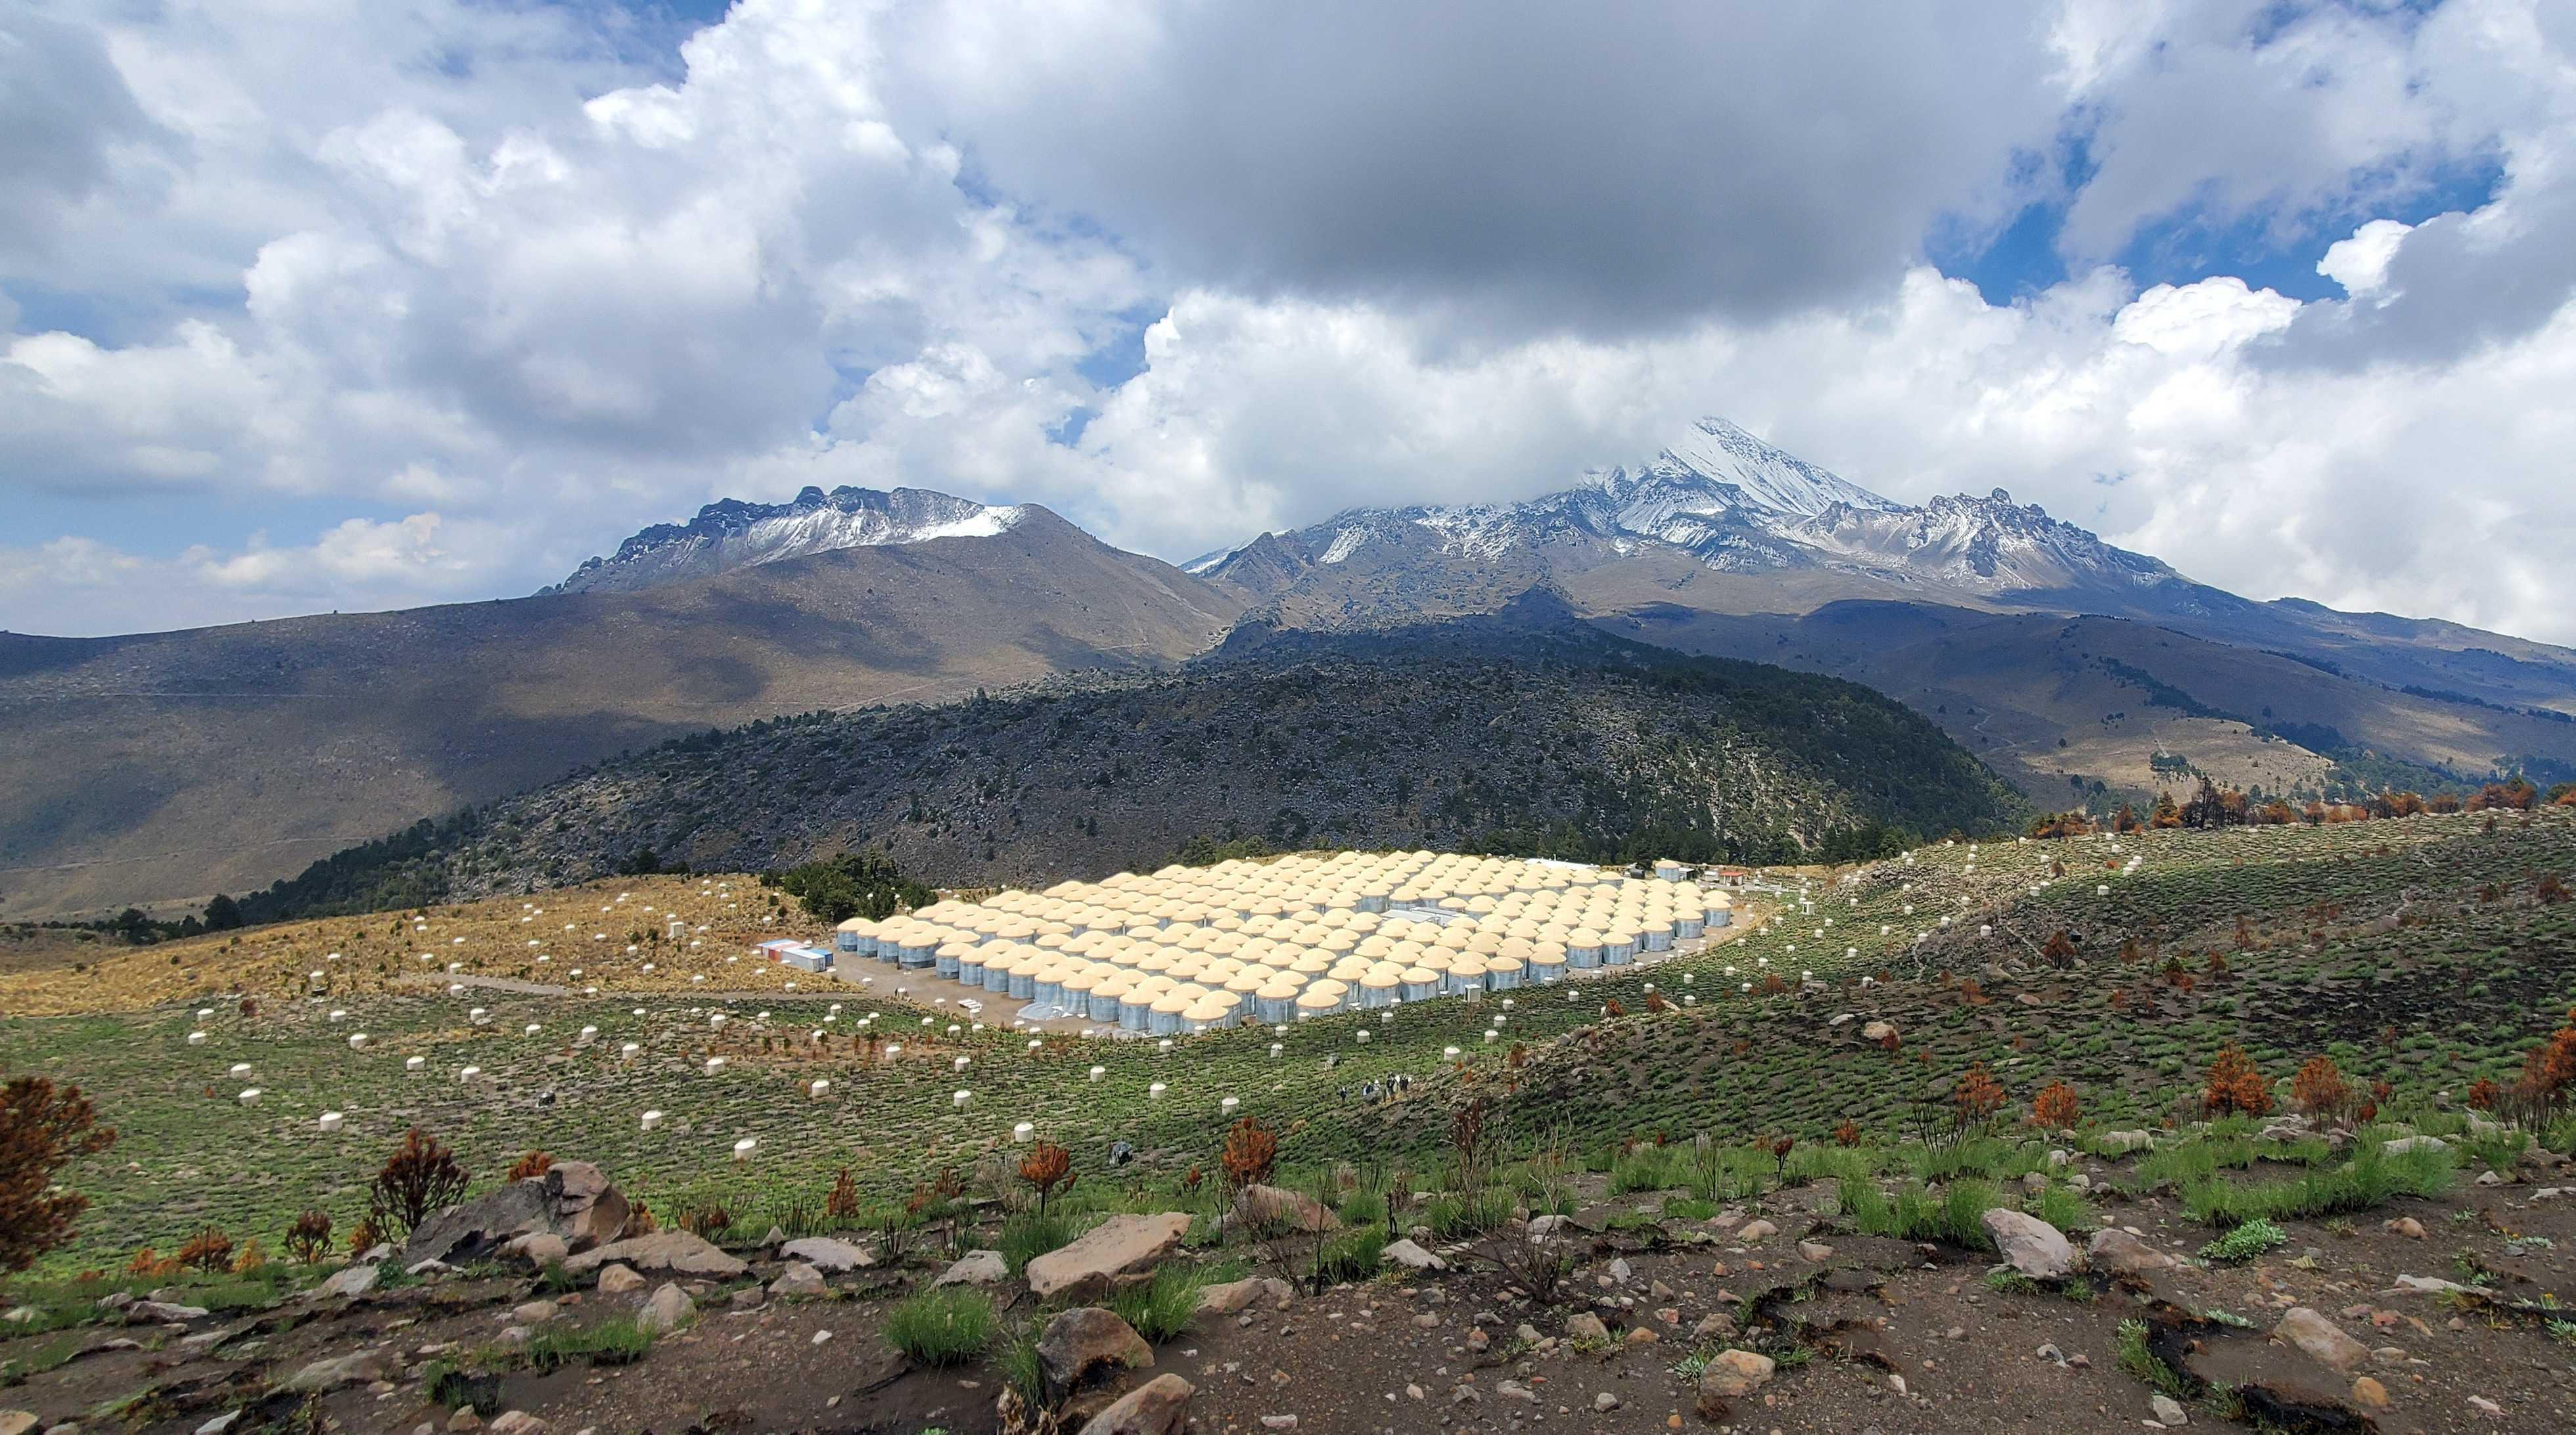
\includegraphics[scale=0.155]{figures/hawc/HAWC.jpg}
    }
    \caption{Photo of the HAWC detector that I took on May 17, 2023. Main array is centered in the photo and comprised of the larger tanks. Outriggers are the smaller tanks around the main array.}
    \label{fig:HAWC}
\end{figure}

The High Altitude Water Cherenkov (HAWC) Observatory is a specialized instrument designed for the observation of high energy gamma-rays and cosmic rays \cite{HAWC_NIM}.
Located on the Sierra Negra volcano in Mexico, HAWC observes gamma rays and cosmic rays in the energy range of approximately 100 GeV to 100's of TeV.
HAWC is strategically situated to maximize observational efficiency due to its high altitude.
At an elevation of 4,100 meters, it monitors about two-thirds of the sky every day with an uptime above 90\%.
This capability is essential for studying high-energy astrophysical phenomena.

HAWC consists of 300 water Cherenkov detectors (WCDs) spread over 22,000 $m^2$.
Each main array detector is filled with purified water and equipped with four, upward-facing photomultiplier tubes (PMTs).
See \cref{fig:WCD_schematic} for schematic of WCDs.
These PMTs detect Cherenkov radiation from charged particles passing through the tanks.
These charged particles are generated when a high energy gamma or cosmic ray collides with gas in the atmosphere to create a charged particle shower, see \cref{fig:airshowers}.
The observatory includes a separate tank configuration which are refered to as the outriggers.
They are a secondary array of 345 smaller WCD's.
Surrounding the main array, each outrigger tank measures 1.55 meters in diameter and height and contain a single upward-facing eight-inch PMT.
This add-on increases the instrumented footprint fourfold.
The outriggers are meant to improve the reconstruction of showers extending beyond the main array, especially for events above 10 TeV.
However, at the time of writing this thesis, the outriggers have not been fully integrated into HAWC's reconstruction software.

\begin{figure}
    \centering{
    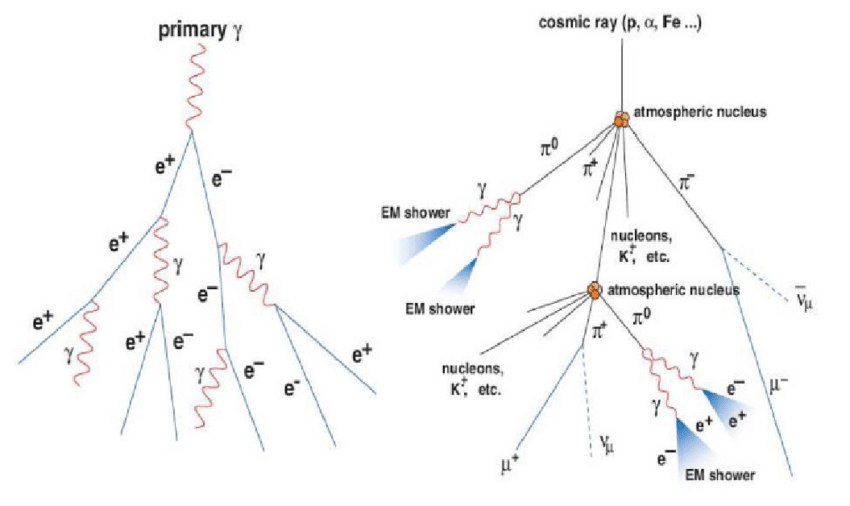
\includegraphics[scale=0.5]{figures/hawc/high_energy_air_shower.png}
    }
    \caption{A particle physics illustration of high energy particle showers. Left shower is an electromagnetic shower from a high energy gamma-ray. Most particles in the shower will be a combination of photons and charged leptons, in this case electrons (e). Right figure shows a cosmic ray particle shower. The cosmic ray will produce many more types of particles including pions ($\pi$), neutrinos, and charged leptons. Figured pulled from \cite{lopez_thesis}.}
    \label{fig:airshowers}
\end{figure}

%-----------------------------------------------------------------------------------%
\subsection{Construction and Hardware} \label{sec:hawc_hardware}
%-----------------------------------------------------------------------------------%

\begin{figure}
    \centering{
        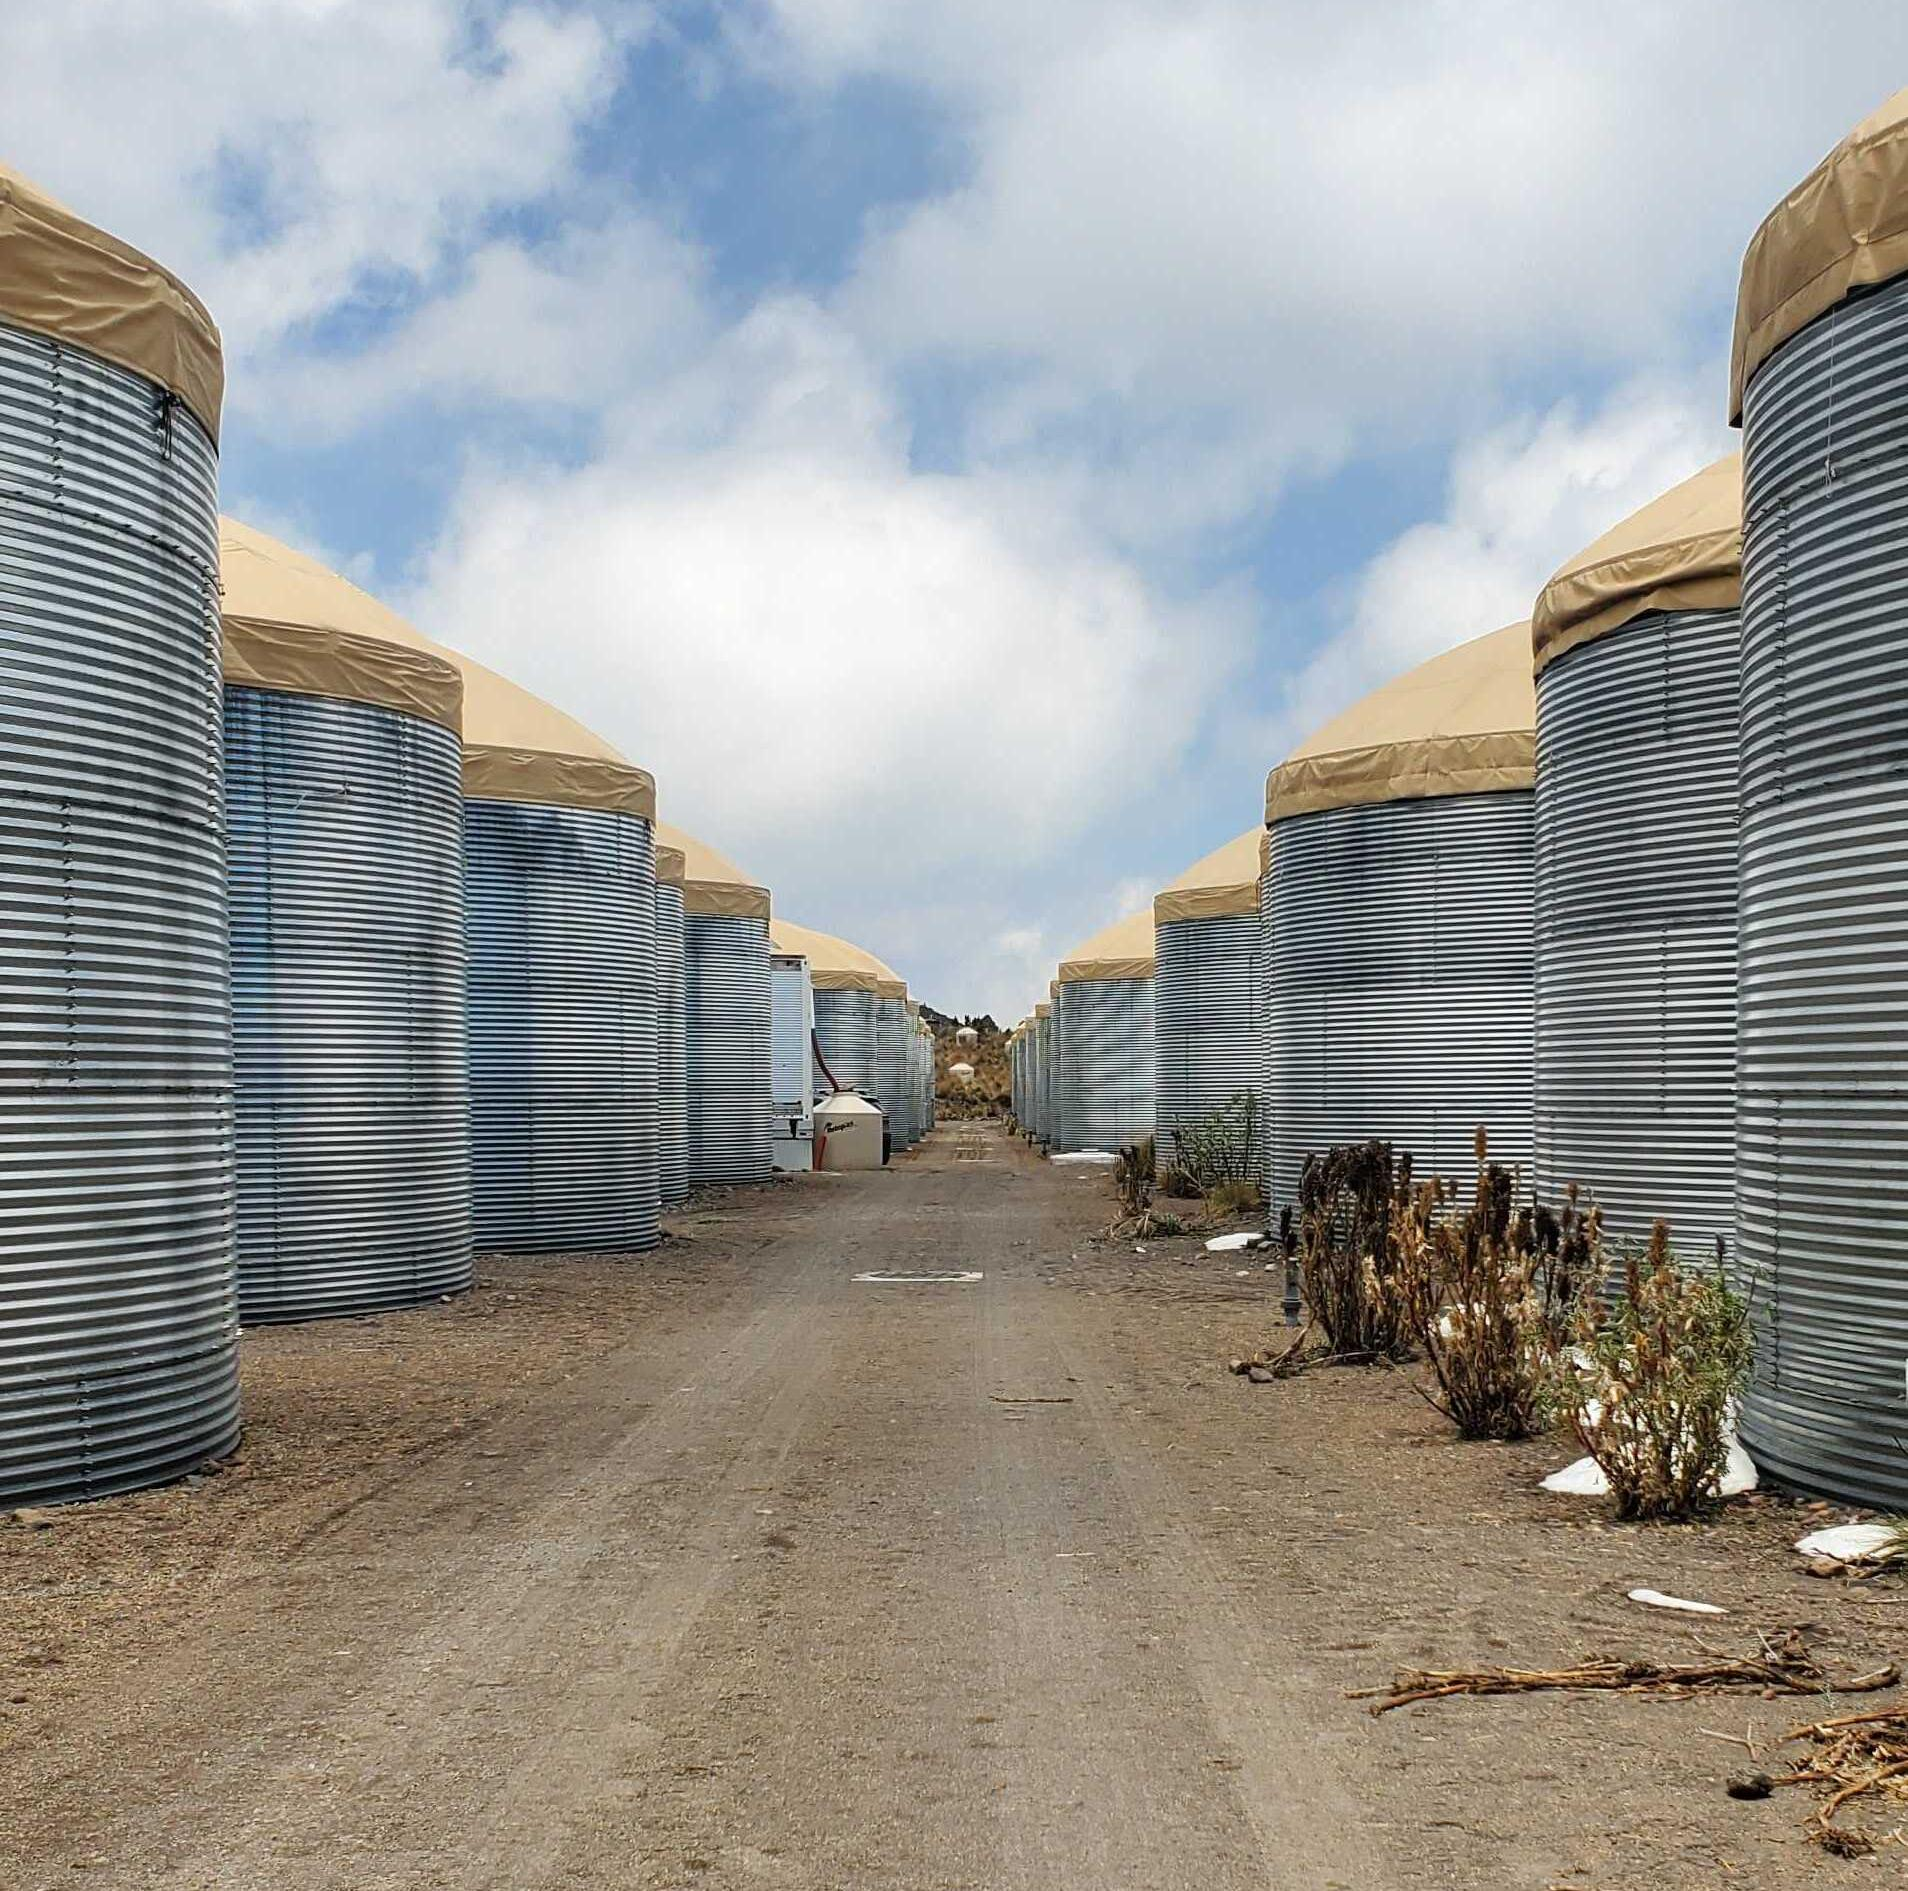
\includegraphics[scale=0.14]{figures/hawc/WCDs.jpg}
        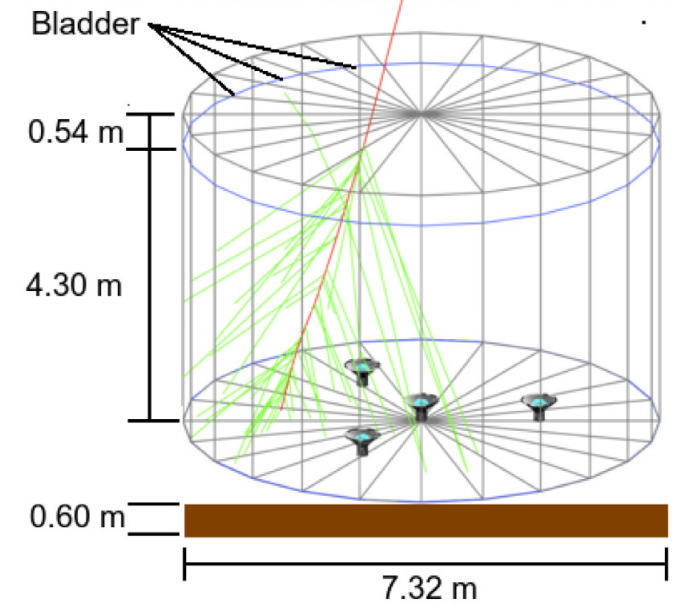
\includegraphics[scale=0.45]{figures/hawc/WCD_schematic.png}
    }
    \caption{The WCDs. Left image features several WCDs looking from within the main array of HAWC. Right image shows a schematic of a WCD pulled from \cite{HAWC_NIM}.}
    \label{fig:WCD_schematic}
\end{figure}

Each main array WCD, see \cref{fig:WCD_schematic}, is a cylindrical tank with dimensions of 7.3 m in diameter and 5.4 m in height and filled with 180,000 L of water \cite{HAWC_NIM}.
The metal shell of these tanks is made from bolted together, corrugated, galvanized steel panels.
The tanks are placed into 0.6 m deep trenches filled with rammed earth to secure it against seismic activity \cite{HAWC_NIM}.
The interior of each tank is lined with a black, low-density polyethylene bladder, designed to be impermeable to external light and to prevent reflection of Cherenkov light within the tank.
This bladder is approximately 0.4 mm thick and composed of two layers of three-substrate film.
To further minimize light penetration, a black agricultural foil covers the bladder.
The ground and walls inside the tank are protected with felt and sand to safeguard against punctures.
The tanks are filled 4.5 m deep of purified water, achieving a photon attenuation length for Cherenkov photons that exceeds the tank's dimensions \cite{HAWC_NIM}.
This purification level ensures the optimal detection environment for the photons generated by traversing charged particles.

At the base of each tank, four photomultiplier tubes (PMTs) are installed to detect the Cherenkov radiation emitted by charged particles in watre.
Three 8-inch diameter PMTs surround a larger 10 inch PMT from Hamamatsu \cite{hawc_pmt}.
The variation in PMT response is carefully accounted for in event reconstruction algorithms.
Signals from the PMTs traverse 610 ft cables to the counting house, where they are processed by Front-End Boards (FEBs), see \cref{fig:basic_tanks_schem,fig:dig_schem}.
These FEBs, along with Time to Digital Converters (TDCs), digitize the signals and manage the high voltage supply to the PMTs.

%-----------------------------------------------------------------------------------%
\subsection{Data Acquisition and Signal Processing} \label{sec:hawc_daq}
%-----------------------------------------------------------------------------------%

\begin{figure}
    \centering{
        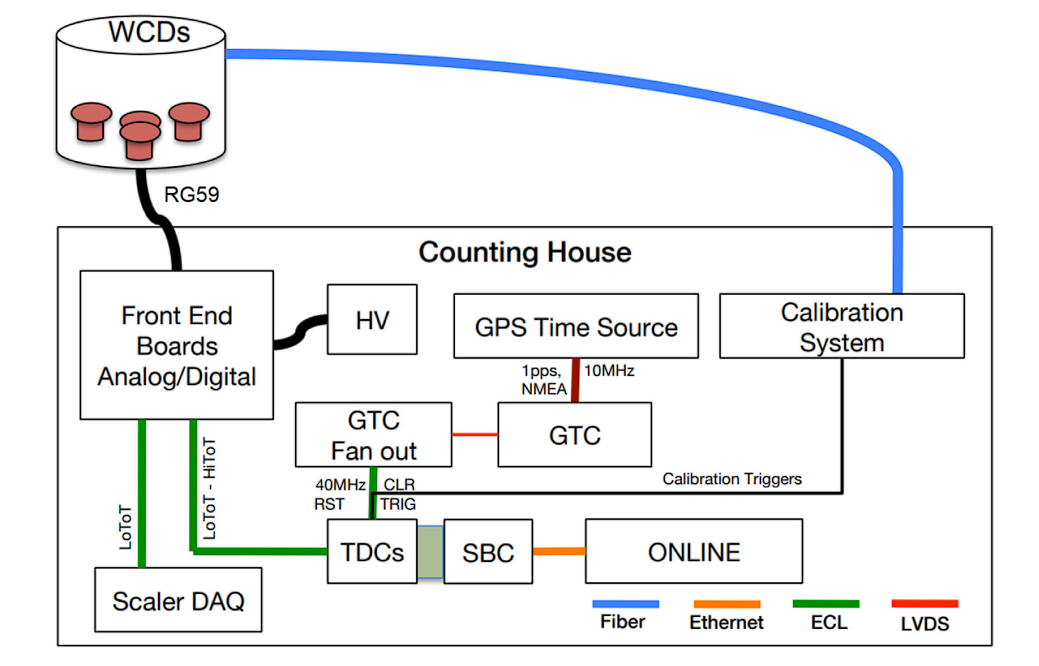
\includegraphics[scale=0.5]{figures/hawc/tank_basic_schem.png}
    }
    \caption{Overview of HAWC control and data electronics. The LoToT and HiToT threshold signals are discussed in \cref{sec:hawc_daq}. Figure from \cite{HAWC_NIM}}
    \label{fig:basic_tanks_schem}
\end{figure}

\begin{figure}
    \centering{
        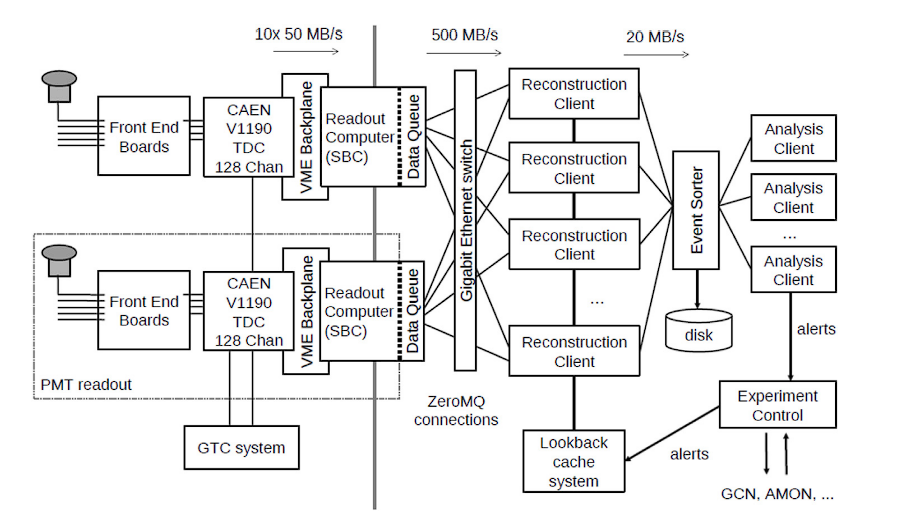
\includegraphics[scale=0.6]{figures/hawc/digital_schematic.png}
    }
    \caption{Schematic of data flow in HAWC data acquisition and online processing system. Pulled from \cite{HAWC_DAQ_NIM}.}
    \label{fig:dig_schem}
\end{figure}

The HAWC data acquisition (DAQ) and signal processing systems convert the physical detection of particles into analyzable data.
This process involves a series of steps from initial signal detection by PMTs to digital conversion and preliminary analysis, see \cref{fig:dig_schem,fig:tot_threholds}.

\begin{figure}
    \centering{
        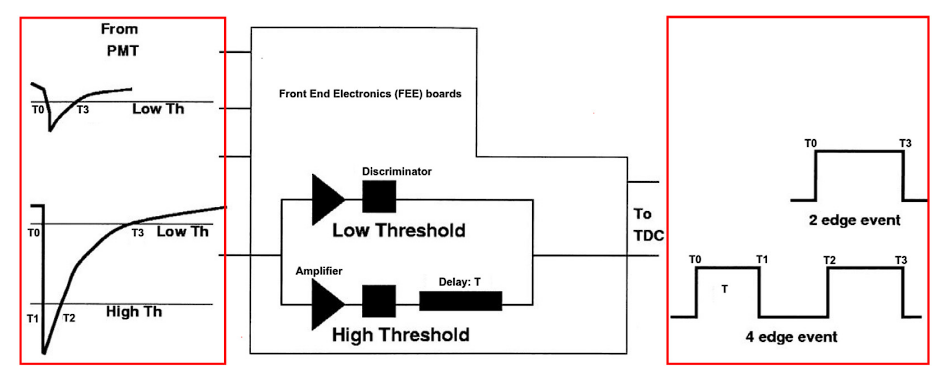
\includegraphics[scale=0.6]{figures/hawc/ToT_threshold.png}
    }
    \caption{How HAWC FEB intially processes analog PMT signals. Signals are split through an amplifier and discriminator circuit. Each path is designated for either the HIGH or LOW threshold for the signal. The 2-edge event corresponds to LOW, while the 4 edge corresponds to HIGH.}
    \label{fig:tot_threholds}
\end{figure}

Once the signal from the PMTs arrive at the counting house, they enter the Front-End Boards (FEBs).
The FEBs are responsible for the initial processing of these signals, which includes amplification and integration \cite{Milagro_DAQ}.
Each PMT signal is compared against preset LOW/HIGH voltage thresholds in the FEBs, see \cref{fig:tot_threholds}, identifying signals that correspond to about 1/4 and 4 photoelectrons, respectively.
This differentiation allows the system to gauge the strength of the detected Cherenkov radiation.
The processed signals are then digitized by Time to Digital Converters (TDCs).
These converters measure the time over threshold (ToT) for each signal, a parameter that reflects both the duration and amplitude of the signal.
This digitization facilitates reconstruction of the original event for translating the physical interactions within the detectors into data \cite{HHAWC_NIM,HAWC_DAQ_NIM,Milagro_DAQ}.

Synchronization across the HAWC observatory is maintained by a central GPS Timing and Control (GTC) system, which achieves a timing resolution of 98 ps.
This high-resolution timing is vital for accurately reconstructing the timing and location of air showers initiated by cosmic and gamma rays.
The GTC system ensures that all components of the DAQ operate in unison to preserve the temporal integrity of the detected events \cite{HHAWC_NIM,hawc_daq_thesis}.

Once digitized, the data are transferred to an online event reconstruction system.
This system runs the Reconstruction Client, which utilizes the raw PMT data to reconstruct the characteristics of the air showers, such as their direction and energy \cite{HAWC_DAQ_NIM}.
The capacity for real-time analysis allows HAWC to promptly respond to astrophysical phenomena like Gamma Ray Bursts (GRBs) and to participate in multi-messenger astronomy by following up on alerts from other observatories.
This real-time processing system is designed to handle high data throughput, using ZeroMQ \cite{zeromq} for efficient data transfer between software components.
Analysis Clients perform specific online analyses that require immediate data, including monitoring for GRBs, solar flare activity, and participation in global efforts to track gravitational waves and neutrinos \cite{HAWC_NIM}.

The DAQ system is overseen by an Experiment Control system and crew that manage the operational aspects of data collection.
This includes initiating and terminating data collection runs and monitoring the experiment for errors.
In the event of a system crash, often caused by environmental factors such as lightning, the Experiment Control system is designed to automatically restart the experiment and minimize downtime \cite{HAWC_NHAWC_NIM,HAWC_DAQ_NIM}.

%-----------------------------------------------------------------------------------%
\section{Event Reconstruction} \label{sec:hawc_reconstruction}
%-----------------------------------------------------------------------------------%

Event reconstruction at the HAWC Observatory is a critical procedure that converts the raw data from the observatory's WCDs into a coherent framework for understanding cosmic and gamma-ray events.
This process includes several distinct steps.
Core Fitting determines the geometric center of the air shower on the detector plane.
Angle Reconstruction assesses the trajectory of the incoming particle, revealing its origin in the sky.
Energy Estimation is performed using both \textit{f}-hit and Neural Network (NN) methods to quantify the energy of the detected events.
Gamma/Hadron discrimination differentiates between gamma-ray and hadronic cosmic ray initiated showers, a vital step for astrophysical interpretations.
Each of these steps is integral to the observatory's objective of investigating the high-energy universe and enable the transformation of signals into detailed insights about high energy cosmic phenomena.

%$$$$$$$$$$$$$$$$$$$$$$$$$$$$$$$$$$$$$$$$$$$$$$$$$$$$$$$$$$$$$$$$$$$$$$$$$$$$$$$$$$$%
\subsection{Core Fitting} \label{sec:hawc_core_fitting}
%$$$$$$$$$$$$$$$$$$$$$$$$$$$$$$$$$$$$$$$$$$$$$$$$$$$$$$$$$$$$$$$$$$$$$$$$$$$$$$$$$$$%

\begin{figure}[h!]
    \centering{
    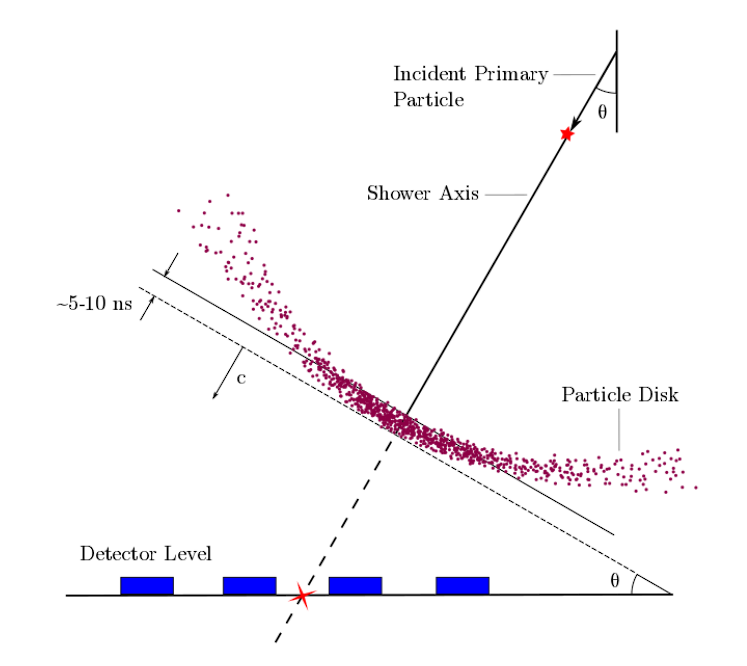
\includegraphics[scale=0.5]{figures/hawc/shower_shape.png}
    }
    \caption{An particle shower incident on WCDs. Secondary particles of an air shower travel in a cone centered on primary incident particle. Reconstruction of the initial angle is possible with arrival time of hits in PMTs inside WCDs. Figure from \cite{thesis_Zigg}.}
    \label{fig:shower_shape}
\end{figure}

In the study of air showers, accurately determining the location of the air shower core on the ground is crucial for reconstructing the direction of the originating primary particle.
An illustration of this can be seen in a HAWC event plot, \cref{fig:airshowers,fig:ldf_particleshower}, where the lateral charge distribution across the array is displayed.
The core is identified and marked with a red star, reconstructed using a predetermined functional form, \cref{eq:hawc_showercore}.

We model signal $S_i$ from the \textit{i}th PMT is given by the following equation:
\showercore
In this model, $\tilde{x}$ represents the core location and $\tilde{x}_i$ is the position of the \textit{i}th PMT.
$R_m$ stands for the Molière radius, which is approximately 120 meters at the altitude of HAWC.
$\sigma$ is the standard deviation of the Gaussian distribution.
$N$ is the normalization factor for the tail of the distribution.
The equation incorporates fixed values of $\sigma = 10$ m and $N=5.10^{-5}$.
This leaves the core location and overall amplitude $A$ as the free parameters to be determined during fitting.

\begin{figure}
    \centering{
        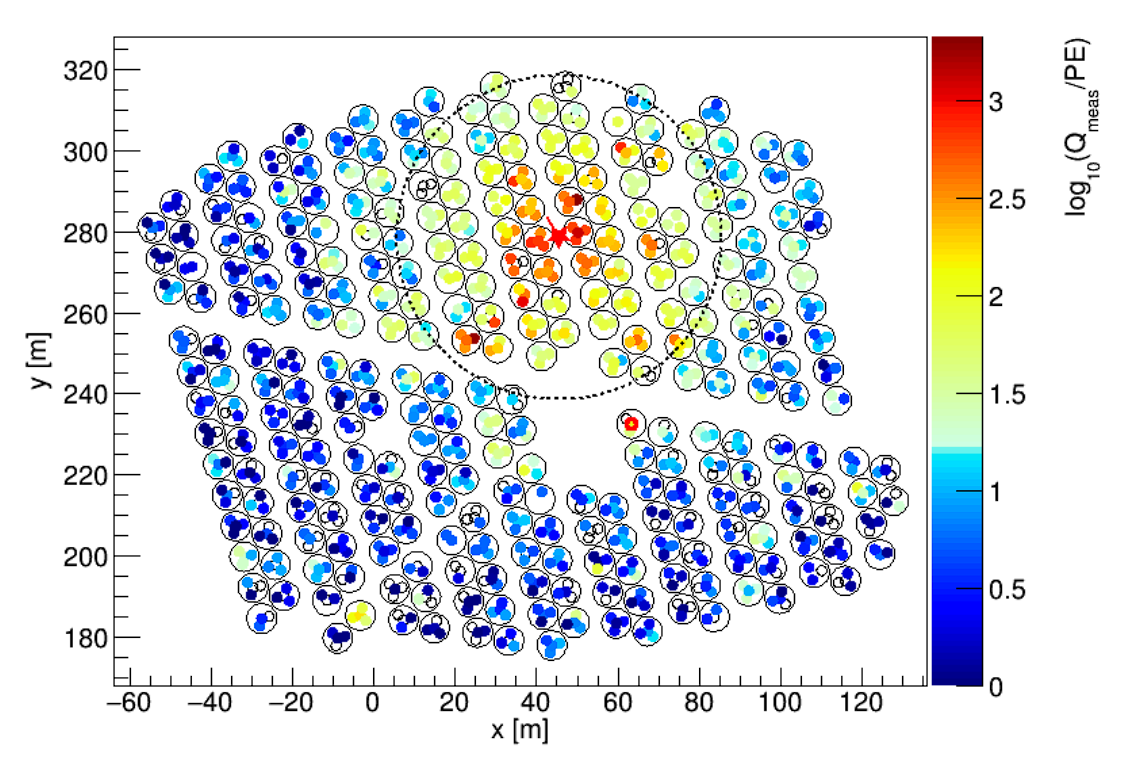
\includegraphics[scale=0.5]{figures/hawc/core_fitting.png}
    }
    \caption{Charge deposition in each PMT for a reconstructed gamma-ray event. WCDs are outlined in black surrounding the 4 smaller circles that represent PMTs. The color scale indicates the charge deposition in each PMT. The best shower core fit from SFCF is noted with a red star in the center of the dashed circle \cite{Abeysekara_2017}.}
    \label{fig:core_fitter}
\end{figure}

The chosen functional form for the Super Fast Core Fit (SFCF) algorithm is a simplified version of a modified Nishimura-Kamata-Greisen (NKG) function \cite{cosmic_ray_shape}, selected for its computational efficiency which is essential for rapid fitting of air shower cores.
The SFCF form allows numerical minimization to converge more quickly due to the function's simplicity, the analytical computation of its derivatives, and the absence of a pole at the core location \cite{Abeysekara_2017}.
\Cref{fig:core_fitter} provides a visualization of a recorded event, with the plot depicting the charge recorded by each PMT as a function of the distance to the reconstructed shower core.
Through the application of the SFCF, core locations can be identified with a median error of approximately 2 m for large events and about 4 m for smaller ones, assuming the gamma-ray event core impacts directly upon the HAWC detector array \cite{Abeysekara_2017}.
It is noted that as the core's distance from the main array increases, the precision in locating the core diminishes \cite{Abeysekara_2017}, highlighting the importance of proximity in the accuracy of core reconstruction.


%$$$$$$$$$$$$$$$$$$$$$$$$$$$$$$$$$$$$$$$$$$$$$$$$$$$$$$$$$$$$$$$$$$$$$$$$$$$$$$$$$$$%
\subsection{Angle Reconstruction} \label{sec:hawc_angleReco}
%$$$$$$$$$$$$$$$$$$$$$$$$$$$$$$$$$$$$$$$$$$$$$$$$$$$$$$$$$$$$$$$$$$$$$$$$$$$$$$$$$$$%

After establishing the core position, the next step is angle reconstruction.
This process determines the primary particle's trajectory.
The angle of arrival is indicative of the originating gamma ray's direction.
It correlates to the cosmic source of the gamma-ray.
We deduce this angle using the timing of PMT hits \cite{Abeysekara_2017}.

The air shower's front is conically shaped, not flat.
This shape arises from the travel patterns of secondary particles.
An event example is illustrated in \cref{fig:shower_shape}.
Far from the core, secondary particles undergo multiple scattering.
They also travel longer distances \cite{wcd_Sensitivity}.
Particle sampling decreases with distance from the core.
This decrease results in measurable delays in arrival times \cite{wcd_Sensitivity,Abeysekara_2017}.
Simulations provide a corrective measure for these effects.
The correction is a function of shower parameters \cite{Abeysekara_2017}.
It adjusts both curvature and sampling.
The distance from the shower core and the charge recorded by PMTs are crucial to this correction.
A function based on simulation and Crab Nebula observations is used for this purpose \cite{Abeysekara_2017}.
This curvature correction allows us to fit the particle front as a plane wave.

Corrections lead to the $\chi^2$ minimization step.
This technique fits a plane to the timing data of the PMTs.
It then calculates the shower's angle of arrival.
The zenith and azimuth angles are the results of this fit \cite{wcd_Sensitivity}.
The local angles are converted to celestial coordinates.
These coordinates allow correlation with gamma-ray sources.
Right ascension (RA) and declination (Dec) are used for this purpose.
RA is akin to longitude, and Dec to latitude.

The reconstructed angle's resolution ranges from 0.1° to 1°.
This range depends on the incoming particle's energy and zenith angle \cite{wcd_Sensitivity}.
The analysis uses a curvature/sampling correction.
This correction applies a quadratic function based on distance from the core \cite{Abeysekara_2017}.
The adjustment improves angular resolution.
However, discrepancies between simulation and observation persist.
These discrepancies introduce systematic errors into HAWC analyses \cite{Abeysekara_2017}.

%$$$$$$$$$$$$$$$$$$$$$$$$$$$$$$$$$$$$$$$$$$$$$$$$$$$$$$$$$$$$$$$$$$$$$$$$$$$$$$$$$$$%
\subsection{$f_\mathrm{hit}$ Energy Estimation}\label{sec:hawc_fhit}
%$$$$$$$$$$$$$$$$$$$$$$$$$$$$$$$$$$$$$$$$$$$$$$$$$$$$$$$$$$$$$$$$$$$$$$$$$$$$$$$$$$$%

\begin{figure}
    \centering{
        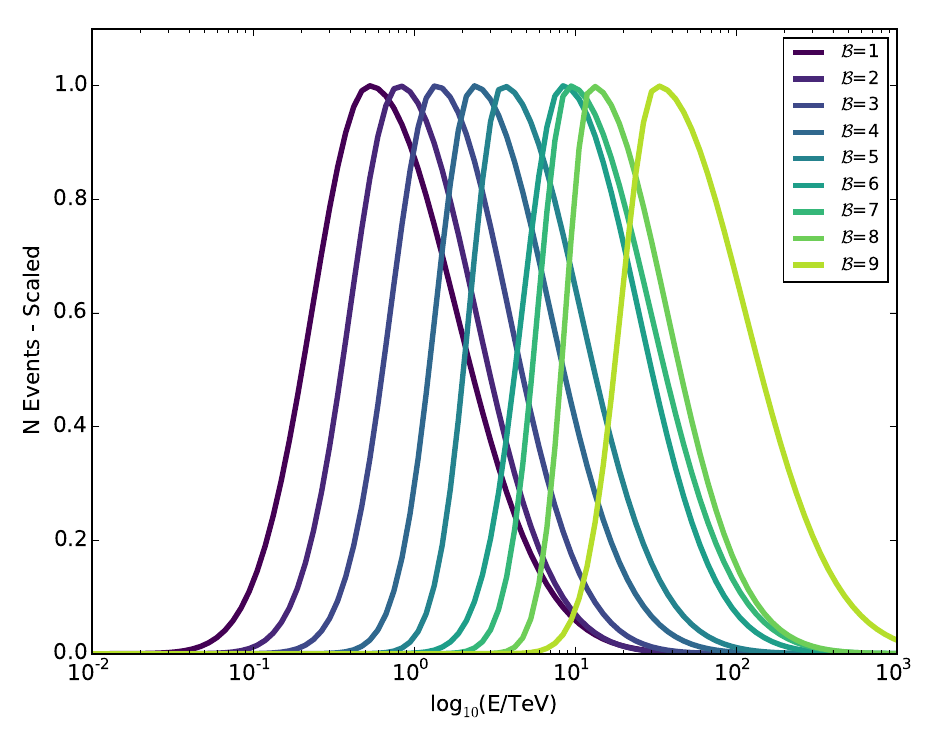
\includegraphics[scale=0.6]{figures/hawc/fhit_bins.png}
    }
    \caption{Simulated normalized energy distribution of each $f_\mathrm{hit}$ bin defined in \cref{tab:fhit_bins}. Monte Carlo simulation of gamma-rays with $E^-{2.63}$ spectral shape and simulated source at 20$^\circ$ declination. Figure from \cite{Abeysekara_2017}.}
    \label{fig:fhit_bins}
\end{figure}

\begin{table}
    \centering{
    \begin{tabular}{c?cc|c}
        \hline
        Bin &
        Lower Edge \% &
        Upper Edge \% &
        $\Theta_{68}$ ($^\circ$) \\
        \hline
        1       &
        6.7     &
        10.5    &
        1.05    \\

        2       &
        10.5    &
        16.2    &
        0.69    \\

        3       &
        16.2     &
        24.7    &
        0.50    \\

        4       &
        24.7     &
        35.6    &
        0.39    \\

        5       &
        35.6     &
        48.5    &
        0.30    \\

        6       &
        48.5     &
        61.8    &
        0.28    \\

        7       &
        61.8     &
        74.0    &
        0.22    \\

        8       &
        74.0     &
        84.0    &
        0.20    \\

        9       &
        84.0     &
        100    &
        0.17    \\

    \end{tabular}
    }
    \caption{Definitions of $f_\mathrm{hit}$ energy estimator bins. Bins are defined by the fraction of available PMTs that are triggered during an air shower event. The angular resolution, $\Theta_{68}$, is the bin containing 68\% of events \cite{Abeysekara_2017}.}
    \label{tab:fhit_bins}
\end{table}

The HAWC Observatory quantifies the primary particle energy of air showers using a metric known as $f_{\text{hit}}$.
This ratio compares the count of PMTs involved in the event reconstruction to the total number of functional PMTs at the time \cite{Abeysekara_2017}.
The main array consists of about 1200 PMTs, but the count may vary due to maintenance or other operational factors.

Events are stratified into several $f_{\text{hit}}$ bins.
Each bin corresponds to a specific range of angular resolutions, enabling a structured approach to event analysis based on the extent of the shower footprint, see \cref{tab:fhit_bins}.
The $f_{\text{hit}}$ metric, while effective, has several limitations.
It is dependent on the zenith angle and the spectral characteristics presumed for the observed source.
The variable also reaches a saturation point around 10 TeV, after which the detector's ability to discriminate between higher energy levels diminishes \cite{Abeysekara_2017}.
Furthermore, the energy distribution for each $f_{\text{hit}}$ bin is notably broad, see \cref{fig:fhit_bins}.
In response to these limitations, HAWC has developed more intricate algorithms for energy estimation.
These algorithms incorporate the zenith angle and the distribution of charge around the shower core for a more accurate assessment of the primary particle's energy, particularly at energies surpassing 10 TeV \cite{wcd_Sensitivity}.

The relationship between $f_{\text{hit}}$ and primary energy is complex.
Atmospheric attenuation can cause high-energy showers to present a smaller footprint, misrepresenting their energy in the $f_{\text{hit}}$ metric.
This effect is captured in simulations that chart the actual energy distribution across $f_{\text{hit}}$ categories \cite{wcd_Sensitivity}.
Such distributions vary with the declination of the source and the theoretical energy spectrum used in the model.

%$$$$$$$$$$$$$$$$$$$$$$$$$$$$$$$$$$$$$$$$$$$$$$$$$$$$$$$$$$$$$$$$$$$$$$$$$$$$$$$$$$$%
\subsection{Neural Network Energy Estimation}\label{sec:hawc_nn}
%$$$$$$$$$$$$$$$$$$$$$$$$$$$$$$$$$$$$$$$$$$$$$$$$$$$$$$$$$$$$$$$$$$$$$$$$$$$$$$$$$$$%

\begin{figure}
    \centering{
        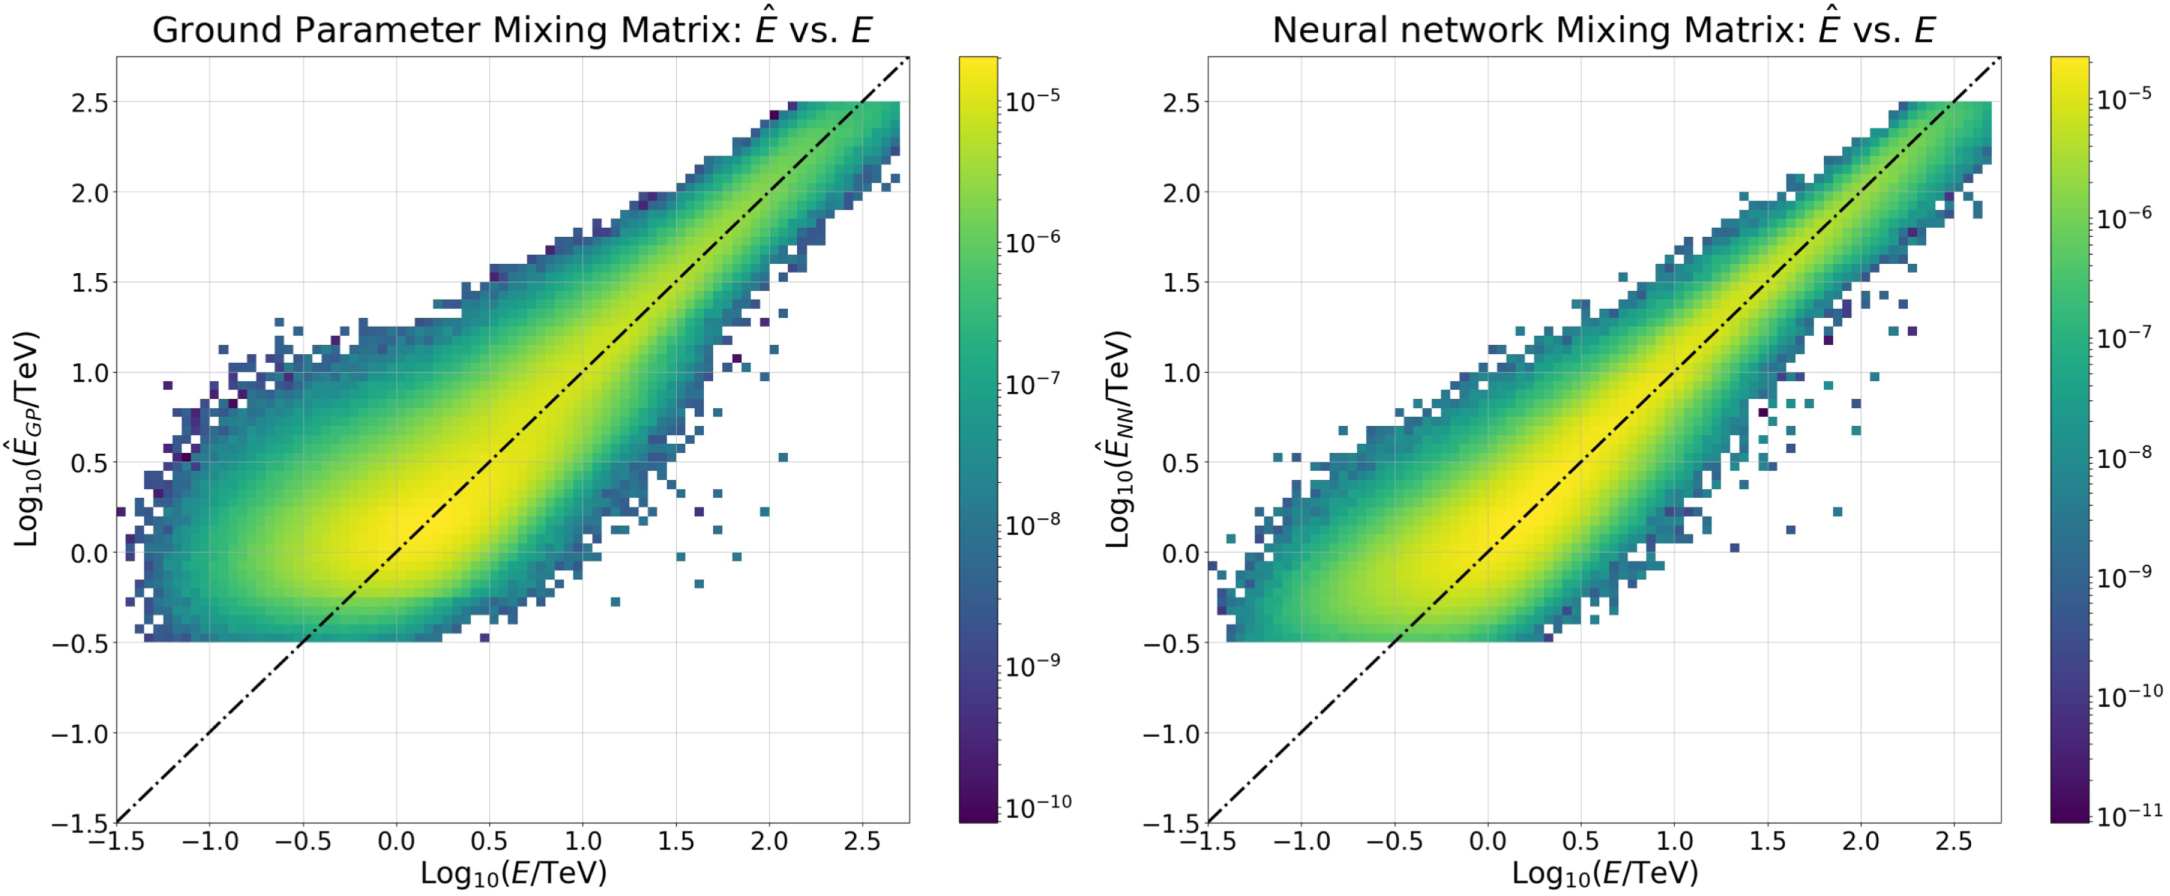
\includegraphics[clip, trim=9.1cm 0cm 0cm 0cm, scale=0.9]{figures/hawc/NN_performance.jpg}
    }
    \caption{Neural Network energy estimator performance compared to true energy. The dotted line is the identity line where the estimator and injection agree. Gamma/hadron separation cuts were applied with the energy estimation. Figure pulled from \cite{100TEV_Crab_HAWC}}
    \label{fig:NN_performance}
\end{figure}

The energy estimation for photon events at the HAWC Observatory is refined through an artificial neural network (NN) algorithm.
This method, based on the Toolkit for Multivariate Analysis NN, adopts a multilayer-perceptron model with logistic activation functions across its layers.
The structure includes two hidden layers, the first with 15 nodes and the second with 14, designed to process input variables through a neural network optimized to estimate primary particle energies \cite{thesis_SamM}.

The NN is trained to minimize a specific error function that measures discrepancies between the NN's energy predictions and the actual energies from Monte Carlo simulations.
This minimization targets an error function that incorporates the relative importance of each event, weighting more the importance to mimic an $E^{-2}$ power law spectrum.
This approach helps achieve a uniform error rate across energies ranging from 1 to 100 TeV.
The optimization process leverages the Broyden-Fletcher-Goldfarb-Shanno algorithm that calibrates the NN's 479 weights \cite{100TEV_Crab_HAWC}.

The spectral analysis employs a binned likelihood method, using a forward-folding technique to accommodate the energy estimate's bias and resolution \cite{100TEV_Crab_HAWC}.
This establishes a 2D binning scheme that categorizes events by both their $f_{\text{hit}}$ value and estimated energy.
The decision to use this scheme over a simple energy-based binning lies in the correlation between gamma/hadron separation parameters and the angular resolution with both the size and energy of the event.
The spectrum of interest is partitioned into nine $f_{\text{hit}}$ bins, each further divided into 12 energy bins, spanning from 0.316 TeV to 316 TeV, encompassing a total of 108 bins \cite{100TEV_Crab_HAWC}.
However, not all bins contribute to the final estimate.
Bins with low event populations or insufficient Monte Carlo simulation are excluded.
This approach focuses on the central 99\% of events by estimated energy within each $f_{\text{hit}}$ bin, effectively removing outliers \cite{100TEV_Crab_HAWC}.

Input variables for the NN are selected to capture key characteristics of the air shower: energy deposition, containment, and atmospheric attenuation.
The algorithm calculates energy deposition using the fraction of PMTs and tanks activated, alongside the logarithm of the normalization from the lateral distribution fit.
Containment is inferred from the distance between the shower core and the array's center, while atmospheric attenuation is evaluated using the reconstructed zenith angle and a detailed analysis of the shower's lateral charge distribution \cite{thesis_SamM,100TEV_Crab_HAWC}.

This refined NN energy estimation methodology is an integral component of HAWC's toolkit, enabling precise analysis of high-energy gamma-ray events.
It represents a significant advancement in the field by more accurately mapping observed shower characteristics to primary particle energies.

%$$$$$$$$$$$$$$$$$$$$$$$$$$$$$$$$$$$$$$$$$$$$$$$$$$$$$$$$$$$$$$$$$$$$$$$$$$$$$$$$$$$%
\subsection{G/H Discrimination}\label{hawc:gammaHadron}
%$$$$$$$$$$$$$$$$$$$$$$$$$$$$$$$$$$$$$$$$$$$$$$$$$$$$$$$$$$$$$$$$$$$$$$$$$$$$$$$$$$$%

\begin{figure}
    \centering{
        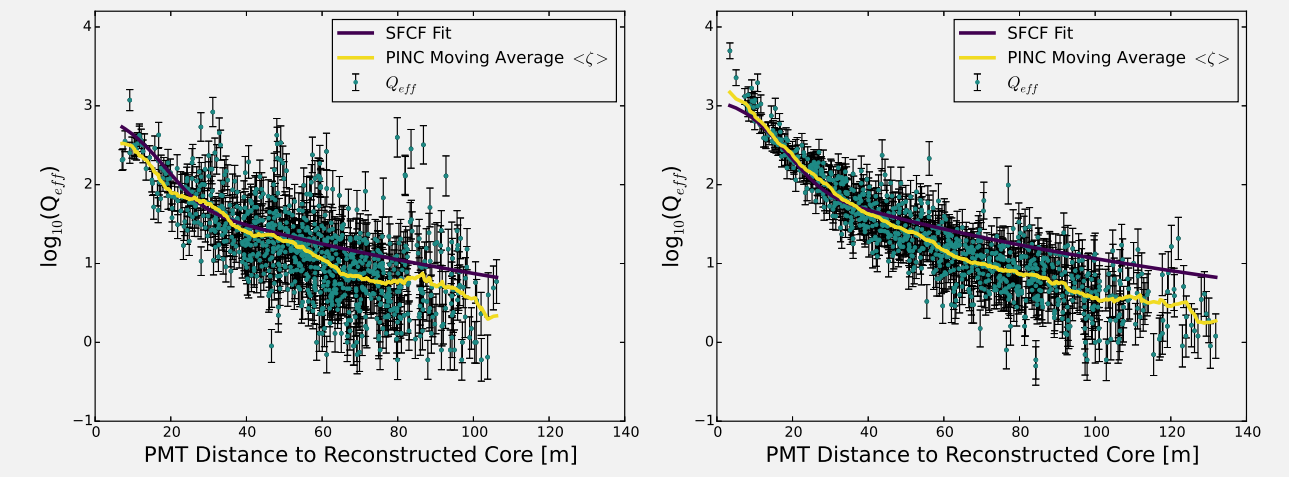
\includegraphics[scale=0.45]{figures/hawc/LDF_particles.png}
    }
    \caption{Lateral distribution functions (LDFs) for cosmic ray (left) and a photon candidate from the Crab Nebula (right). Cosmic ray LDF has clearly isolated hits far from the reconstructed shower core. Gamma-ray shower shows a more cuspy event \cite{Abeysekara_2017}.}
    \label{fig:ldf_particleshower}
\end{figure}

At the HAWC Observatory, distinguishing between air showers initiated by gamma rays and those by hadronic cosmic rays is fundamental for astrophysical data purity.
The separation process leverages differences in shower characteristics: electromagnetic showers from gamma rays typically display fewer muons and a smoother lateral distribution, whereas hadronic showers are more chaotic due to the abundance of muons and hadronic sub-showers.

Two primary parameters facilitate the identification of cosmic-ray events \cite{Abeysekara_2017}:

Compactness (C): This parameter evaluates the charge captured by PMTs, particularly focusing on the PMT with the highest effective charge beyond a 40-meter radius from the shower core.
Compactness is inversely proportional to this effective charge, as higher charges at extended distances from the core are indicative of hadronic showers.
It is mathematically expressed as:
\compactness
where $N_\mathrm{hit}$ is the number of PMTs hit and $CxPE_{40}$ is the effective charge measured outside a 40 m radius from the shower cores \cite{Abeysekara_2017}.

PINCness (P): PINCness quantifies the "clumpiness" of a shower using the charges recorded by PMTs and is short for Parameter for Identifying Nuclear Cosmic Rays.
It is computed from the logarithm of the effective charge, $Q_{\mathrm{eff},i}$, of each PMT hit, $i$, compared to an expected average for that annular region.
A higher PINCness suggests a less smooth distribution, typical of hadronic showers.
The formula is:
\pincness
where $\zeta_i = \log_{10}(Q_{\mathrm{eff},i})$.
The average, $\langle \zeta \rangle$ is the average over an anular region surrounding the shower core.
The errors, $\sigma_{\zeta_i}$, are computed and allocated from gamma-ray candidates close to the Crab.

These parameters are tested and modeled in simulations and with observational data near the Crab Nebula.
\Cref{fig:ldf_particleshower} illustrating the lateral distributions for representative cosmic-ray and photon candidate showers, as well as the distribution of these discrimination parameters, affirm their efficacy \cite{Abeysekara_2017}.

The discrimination technique has remained consistent, but cut values have been reoptimized for the 2D bins based on $f_{\text{hit}}$ and NN estimated energy.
This refinement enhances the selection of high-energy events.
Each bin ensures at least 50\% efficiency for gamma-ray detection, with efficiencies extending up to nearly 100\% in certain bins \cite{Abeysekara_2017,100TEV_Crab_HAWC}.

%$$$$$$$$$$$$$$$$$$$$$$$$$$$$$$$$$$$$$$$$$$$$$$$$$$$$$$$$$$$$$$$$$$$$$$$$$$$$$$$$$$$%
\section{Background Estimation: Direct Integration}\label{hawc:direc_int}
%$$$$$$$$$$$$$$$$$$$$$$$$$$$$$$$$$$$$$$$$$$$$$$$$$$$$$$$$$$$$$$$$$$$$$$$$$$$$$$$$$$$%

The ratio of cosmic rays to gamma rays can be as high as 10,000 to 1, depending on the energy.
At HAWC, we confront a significant challenge even after gamma/hadron cuts: our gamma-ray data is still inundated with cosmic-ray events.
To tackle this, we rely on the direct integration method developed by Milagro \cite{Milagro_crab}.
This method capitalizes on the cosmic rays' isotropic nature resulting from their deflection by interstellar magnetic fields.

The direct integration method estimates background events by integrating over a stable two-hour period of detector operation.
The expected number of background events at a particular sky coordinate ($\phi, \theta$) is determined by integrating the normalized detector's efficiency with the all-sky event rate:
\directInt
Here, $E(\text{ha}, \theta)$, represents the detector's efficiency, which varies with local coordinates (hour angle and declination).
$R(t)$ is the event rate as a function of time \cite{Milagro_crab}.

Our background estimation is expected to falter in high-energy ranges where cosmic-ray events are less frequent due to enhanced gamma/hadron discrimination. Sparsity in our background and data also arise at the limits of HAWC's sensitivity and during short-term analyses of transient events.
HAWC addresses these issues by using a pixel size of 0.5$^\circ$ in our direct integration to maintain robustness in our estimation \cite{Abeysekara_2017,wcd_Sensitivity}.
In constructing the background model, it's crucial to exclude areas of the sky with known gamma-ray sources.
Regions containing the Crab Nebula, Mrk 421, Mrk 501, and the Galactic Plane are masked to prevent their significant gamma-ray signals from biasing our background estimate \cite{Abeysekara_2017}.


%%%%%%%%%%%%%%%%%%%%%%%%%%%%%%%%%%%%%%%%%%%%%%%%%%%%%%%%%%%%%%%%%%%%%%%%%%%%%%%%%%%%%
\chapter{IceCube\label{sec:ice3}}
%%%%%%%%%%%%%%%%%%%%%%%%%%%%%%%%%%%%%%%%%%%%%%%%%%%%%%%%%%%%%%%%%%%%%%%%%%%%%%%%%%%%%

%%%%%%%%%%%%%%%%%%%%%%%%%%%%%%%%%%%%%%%%%%%%%%%%%%%%%%%%%%%%%%%%%%%%%%%%%%%%%%%%%%%%%
\chapter{Glory Duck\label{sec:glory_duck}}
%%%%%%%%%%%%%%%%%%%%%%%%%%%%%%%%%%%%%%%%%%%%%%%%%%%%%%%%%%%%%%%%%%%%%%%%%%%%%%%%%%%%%

%%%%%%%%%%%%%%%%%%%%%%%%%%%%%%%%%%%%%%%%%%%%%%%%%%%%%%%%%%%%%%%%%%%%%%%%%%%%%%%%%%%%%
\chapter{Nu Duck\label{sec:nu_duck}}
%%%%%%%%%%%%%%%%%%%%%%%%%%%%%%%%%%%%%%%%%%%%%%%%%%%%%%%%%%%%%%%%%%%%%%%%%%%%%%%%%%%%%

% Your bibliography command here
% e.g. \bibliography{your-bib-file}) if using natbib
% e.g. \printbibliography if using biblatex

\end{document}